\documentclass{article}

% if you need to pass options to natbib, use, e.g.:
%     \PassOptionsToPackage{numbers, compress}{natbib}
% before loading neurips_2019

% ready for submission
%\usepackage[nonatbib]{neurips_2019}
\usepackage{iclr2020_conference,times}
% \usepackage{neurips_2019}
% \usepackage[nonatbib,preprint]{neurips_2019}
% \usepackage[nonatbib,final]{neurips_2019}

\newcommand{\dds}{DDS}

\usepackage[utf8]{inputenc} % allow utf-8 input
\usepackage[T1]{fontenc}    % use 8-bit T1 fonts
\usepackage{nicefrac}       % compact symbols for 1/2, etc.
\usepackage[normalem]{ulem}

\usepackage[linesnumbered,ruled]{algorithm2e}
\usepackage{adjustbox}
\usepackage{mathtools}

\newcommand{\gn}[1]{\textcolor{magenta}{\bf\small [#1 --GN]}}
\newcommand{\gnc}[2]{\textcolor{magenta}{\sout{#1} #2}}
\newcommand{\an}[1]{\textcolor{red}{\bf\small [#1 --AA]}}
\newcommand{\anc}[2]{\textcolor{red}{\sout{#1} #2}}
\newcommand{\paul}[1]{\textcolor{blue}{\bf\small [#1 --PM]}}
\newcommand{\paulc}[2]{\textcolor{blue}{\sout{#1} #2}}
\newcommand{\cw}[1]{\textcolor{brown}{\bf\small [#1 --XW]}}
\newcommand{\hp}[1]{\textcolor{gray}{\bf\small [#1 --HP]}}



\title{Optimizing Data Usage via \\ Differentiable Rewards}

% The \author macro works with any number of authors. There are two commands
% used to separate the names and addresses of multiple authors: \And and \AND.
%
% Using \And between authors leaves it to LaTeX to determine where to break the
% lines. Using \AND forces a line break at that point. So, if LaTeX puts 3 of 4
% authors names on the first line, and the last on the second line, try using
% \AND instead of \And before the third author name.
\usepackage{authblk}

\iclrfinalcopy

\author[*,1]{\textbf{Xinyi Wang}}
\author[*,1,2]{\textbf{Hieu Pham}}
\author[1]{\textbf{Paul Michel}}
\author[1]{\textbf{Antonios Anastasopoulos}}
\author[1]{\textbf{Graham Neubig}}
\author[1]{\textbf{Jaime Carbonell}}
\affil[1]{Language Technology Institute, Carnegie Mellon University, Pittsburgh, PA 15213, USA}
\affil[2]{Google Brain, Mountain View, CA 94043, USA}
%\affil[3]{Monash University, Clayton VIC 3800, Australia}
\affil[ ]{\texttt{\{xinyiw1,hyhieu,pmichel1,aanastas,gneubig,jgc\}@cs.cmu.edu}}

%\author{%
  % examples of more authors
  % \And
  % Coauthor \\
  % Affiliation \\
  % Address \\
  % \texttt{email} \\
  % \AND
  % Coauthor \\
  % Affiliation \\
  % Address \\
  % \texttt{email} \\
  % \And
  % Coauthor \\
  % Affiliation \\
  % Address \\
  % \texttt{email} \\
  % \And
  % Coauthor \\
  % Affiliation \\
  % Address \\
  % \texttt{email} \\
%}

\usepackage{times}
\usepackage{fullpage}
\usepackage{float}
\usepackage{graphicx}
\usepackage{amsmath}
\usepackage[numbers,sort]{natbib}
\usepackage[
  pagebackref,
  pageanchor=true,
  plainpages=false,
  pdfpagelabels,
  bookmarks,
  bookmarksnumbered,
  colorlinks=true,
  citecolor=blue,
  menucolor=green,
%pdfborder=0 0 0,  %removes outlines around hyper links in online display
]{hyperref}
\usepackage{subfigure}
\usepackage{microtype}
\usepackage{url}
\usepackage{amsfonts}
\usepackage{amssymb}
\usepackage{amsthm}
\usepackage{mathrsfs}
\usepackage{tikz}
\usepackage{graphicx}
\usepackage{verbatim}
\usepackage{xcolor}
\usepackage{booktabs}
\usepackage{multirow}
\usepackage{todonotes}
\usepackage{footnote}
\usepackage{wrapfig}
\usepackage{blindtext}
\usepackage{caption}
\usepackage{mwe}
% \usepackage{algorithm}
\usepackage{algorithmic}

\makesavenoteenv{tabular}
\usepackage[toc,page]{appendix}
\usepackage{comment}

\newcommand{\cf}{\textit{c.f.}}
\newcommand{\eg}{\textit{e.g.}}
\newcommand{\ie}{\textit{i.e.}}
\newcommand{\etc}{\textit{etc.}}
\newcommand{\fix}{\marginpar{FIX}}
\newcommand{\new}{\marginpar{NEW}}
\newcommand{\z}{\mathbf{z}}
\newcommand{\Z}{\mathbf{Z}}
\newcommand{\y}{\mathbf{y}}
\newcommand{\Y}{\mathbf{Y}}
\newcommand{\x}{\mathbf{x}}
\newcommand{\X}{\mathbf{X}}
\newcommand{\m}{\mathbf{m}}
\newcommand{\s}{\mathbf{s}}
\newcommand{\h}{\mathbf{h}}
\newcommand{\W}{\mathbf{W}}
\newcommand{\expected}[1]{\textbf{E}\left[ #1 \right]}
\newcommand{\variance}[1]{\textbf{Var}\left[ #1 \right]}
\newcommand{\covariance}[1]{\textbf{Cov}\left[ #1 \right]}
\newcommand{\vectornorm}[1]{\left\| #1 \right\|}
\newcommand{\expo}[1]{\exp{\left( #1 \right)}}
\newcommand{\ABS}[1]{\left| #1 \right|}
\newtheorem{theorem}{Theorem}
\newtheorem{proposition}{Proposition}
\newcommand{\defeq}{\mathrel{\stackrel{\makebox[0pt]{\mbox{\normalfont\tiny def}}}{=}}}

\newcommand{\enas}{ENAS}

\def\prerl{RL pretraining\xspace}
\def\as{active search\xspace}
\def\btheta{\vec{\theta}}
\def\bphi{\vec{h}}
\def\bphii{\vec{h}^{(n)}}
\def\ba{\vec{a}}
\def\bas{\vec{a}^{(k)}}
\def\bb{\vec{b}}
\def\bc{\vec{c}}
\def\bd{\vec{d}}
\def\be{\vec{e}}
\def\bbf{\vec{f}} % ugh, oh well
\def\bg{\vec{g}}
\def\bh{\vec{h}}
\def\bi{\vec{i}}
\def\bj{\vec{j}}
\def\bk{\vec{k}}
\def\bl{\vec{l}}
\def\bm{\vec{m}}
\def\bn{\vec{n}}
\def\bo{\vec{o}}
\def\bp{\vec{p}}
\def\bq{\vec{q}}
\def\br{\vec{r}}
\def\bs{\vec{s}}
\def\bsi{\vec{s}^{(n)}}
\def\bt{\vec{t}}
\def\bu{\vec{u}}
\def\bv{\vec{v}}
\def\bw{\vec{w}}
\def\bx{\vec{x}}
\def\by{\vec{y}}
\def\bz{\vec{z}}
\def\bxi{\bx^{(i)}}
\def\bysi{\by^{(i)*}}

\DeclareMathOperator*{\argmax}{argmax}
\DeclareMathOperator*{\argmin}{argmin}
\begin{document}

\maketitle
{\let\thefootnote\relax\footnote{{*: Equal contributions.}}}

\setcounter{footnote}{0}

\begin{abstract}
To acquire a new skill, humans learn better and faster if a private tutor, based on their current knowledge level, inform them whether they should pay extra attention to a practice problem. Similarly, a machine learning model could potentially be trained more efficiently with instructions on the importance of a training data that dynamically ``adapt'' to its current learning state. Meanwhile, identifying the optimal and dynamic importance measure for training any model is a challenging problem, because in order to quantify the effect of a modification to training data importance at a given time during the training, one needs to wait for the whole training process to finish. 
In this paper, we propose Differentiable Adaptive Weighting~(\dds), a novel method for selecting high-quality training data. We formulate the training data importance weight as a parameterized function that is updated along with the main model being trained. The formulation allows direct differentiation to optimize the adaptive data weight, and we show that the derived update rule is equivalent to Reinforcement Learning update with an intuitive reward function. Without significant computing overhead, \dds~delivers strong and consistent improvements on two modalities. Specifically, on multilingual machine translation, \dds~can dynamically identify which related languages are helpful to improve the translation of another language, leading to consistent improvements over a strong heuristic data selection baseline. On image classification tasks with CIFAR-10 and ImageNet, and with different ranges of data, \dds~can also optimize the importance of different training instances throughout training, leading to consistent improvements over the baselines in all settings.\footnote{We will release the code after the paper get accepted.}

\end{abstract}
\section{\label{sec:intro} Introduction}
%\gn{The new title is long and a little awkward. I actually still like ``Differential Data Selection'' or ``Differential Adaptive Data Weighting,'' what's the benefit of this new one over the previous ones?}

%\gn{I think now the intro is trying too hard to position our work in previous work, as opposed to getting across the main point. We can discuss the fine-grained differences with all of these methods in a related work section, but it'll be important to not overwhelm the readers with information before they can even understand the main point of our paper. I think the previous intro was pretty good in general, but might need to be a little bit modified to cover the most relevant recent works (e.g. \cite{learn_to_teach}).}

%\gn{``Optimizing Training'' in the title is a bit vague. ``Learning to Train Models'' might be better. Just ``Differentiable Data Selection'' may also be good?}

%To train a deep learning model, the standard method is to perform uniform stochastic gradient update steps on batches of training data. However, the data provided can have different quality, structure or domain properties from the test data, which might even deteriorate the model performance. 
While deep learning models are remarkably good at fitting large data sets, their performance is also highly sensitive to the structure and domain of their training data. Training on out-of-domain data can lead to worse model performance, while using more relevant data can assist transfer learning.
%\gn{This comment was commented out, but I still think it's relevant. What problems result from this sensitivity to quality or structural domain properties? For example, ``leading to lower performance when training sets are noisy or out-of-domain''?}
Previous work has attempted to create strategies to handle this sensitivity by selecting subsets of the data to train the model on \citep{jiang-zhai-2007-instance,wang-etal-2017-instance,axelrod2011domain,moore2010intelligent}, providing different weights for each example \citep{importance_weight,learn_reweight}, or changing the presentation order of data \citep{cl_bengio,rl_nmt}.
%Many prior work strive to improve model performance by designing better data usage strategies.
%Research on data filtering has found that removing noisy data, or selecting in-domain or structurally similar data can lead to large improvements in model performance while potentially reducing the training time~\citep{jiang-zhai-2007-instance,wang-etal-2017-instance,axelrod2011domain,foster-etal-2010-discriminative,moore2010intelligent,learn_reweight}.
%Curriculum learning, on the other hand, improves the model performance by presenting the model easy examples first and then moving towards harder examples~\citep{cl_bengio}.
%More broadly, good data usage strategies can benefit transfer learning, where we want to use data from a resource rich task/domain to improve the target task/domain we are interested in.
%For example, while training on data from related high-resource languages is an effective approach for improve the model performance on low-resource languages, identifying the good related languages to use is crucial for a competitive model~\citep{TCS}.   

However, there are several challenges with the existing work on better data usage strategies. Most work data filtering criterion or training curriculum rely on domain-specific knowledge and hand-designed heuristics, which can be sub-optimal. To avoid hand designed heuristics, several works propose to optimize a parameterized neural network to learn the data usage schedule, but most of them are tailored to specific use cases, such as handling noisy data for classification~\citep{mentornet}, learning a curriculum learning strategy for NMT~\citep{rl_nmt}, and actively selecting data for annotation~\citep{learn_active_learn,reinforce_cotrain}.
%\gn{What specific use cases? Just saying ``specific'' doesn't give readers an idea how sub-optimal they are.}.
\cite{learn_to_teach} proposes a more general teacher-student framework that first trains a teacher network to select data that directly optimizes development set accuracy over multiple training runs.
% to determine the training decisions of the student model, including optimizer choice and data filtering choice etc. They optimize the data filtering network with Reinforcement Learning~(RL) using the change in dev set loss as the reward for selecting a data instance.
However, because running multiple runs of training simply to train this teacher network entails an $n$-fold increase in training time for $n$ runs, this is infeasible in many practical settings.
In addition, in preliminary experiments we also found the single reward signal provided by dev set accuracy at the end of training noisy to the extent that we were not able to achieve results competitive with simpler heuristic training methods.


%\gn{I made significant changes here, importantly including citing \cite{learn_reweight}. If there's highly relevant work, it's not very honest to not cite it in the introduction, so I added it here and noted that it has been used for filtering noisy examples. Later in the paper we can explain the differences in more detail, then in the experiments we can note that we beat it handily.}
In this paper, we propose an alternative: a general Reinforcement Learning~(RL) framework for optimizing training data usage by training a \emph{scorer network} that minimizes the model loss on the development set.
We formulate the scorer network as a function of the current training examples only,
%\gn{``training data only'' could be ``current training example''?}
making it possible to re-use the model architecture which is designed and trained for the main task. Thus, our method requires no heuristics and is generalizable to various tasks. To make the scorer adaptive, we perform frequent and efficient updates of the scorer network using a reward function inspired by recent work on learning using data from auxiliary tasks~\citep{cos_sim,meta_aux_learn}, which use the similarity between two gradients as a measure of task relevance.
We propose to use the gradient alignment between the training examples and the dev set as a reward signal for \emph{a parametric scorer network}, as illustrated in Figure \ref{fig:method}. We then formulate our framework as an optimization problem found in many prior works such as meta-learning~\citep{finn2017model}, noisy data filtering~\citep{learn_reweight}, and neural architecture search~\citep{darts}, and demonstrate that our proposed update rules follow a direct differentiation of the scorer parameters to optimize the model loss on the dev set.
Thus we refer to our framework as ``Differentiable Data Selection''~(\dds).

%\begin{wrapfigure}{r}{0.5\textwidth}
\begin{figure}
    \centering
    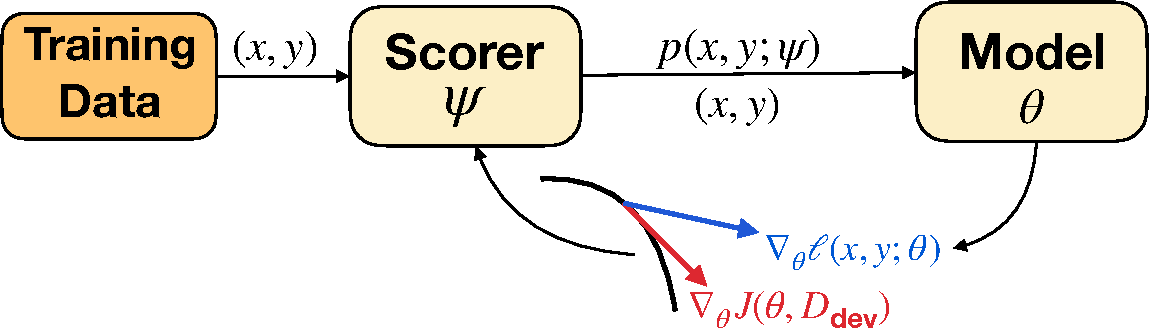
\includegraphics[width=0.4\textwidth]{figs/method_plot_crop.pdf}
    \caption{The general workflow of \dds.}
    \vspace{-0.5cm}
    \label{fig:method}
\end{figure}
%\end{wrapfigure}

We demonstrate two concrete instantiations of the \dds~framework, one for a more general case of image classification, and the other for a more specific case of neural machine translation~(NMT). For image classification, we test on both CIFAR-10 and ImageNet. For NMT, we focus on a multilingual setting, where we optimize data usage from a multilingual corpus to improve the performance on a particular language. % Our contributions are: 1) we propose a general and efficient framework for optimizing training data usage using a teacher network; 2) we provide two specific algorithms for
For these two very different and realistic tasks, we find the \dds~framework brings significant improvements over the baselines for all settings.
\section{\label{sec:method} Differentiable Adaptive Weighting}
\subsection{\label{sec:dds_motivation}Framework}

Commonly in machine learning, we seek to find parameters $\theta$ that minimize the \emph{risk} $J(\theta,P)$, the expected value of a loss function $\ell(x, y; \theta)$, where $\langle x, y \rangle$ are pairs of inputs and associated labels sampled from a particular distribution $P(X, Y)$:
\begin{equation}
  \label{eqn:generic_optim}
   \small
  \begin{aligned}
    \theta^* = \argmin_\theta J(\theta, P)
    ~~~\text{where}~~~
    J(\theta, P) = \mathbb{E}_{x, y \sim P(X, Y)} [\ell(x, y; \theta)]
  \end{aligned}
\end{equation}

In the ideal case, we would like the risk $J(\cdot)$ to be minimized over the inputs and outputs that we will expect our system to see at test time, defined as $P_{\text{test}}(X,Y)$.

To quantify the importance of training data, we propose to replace the distribution $\text{Uniform}(\mathcal{D}_\text{train})$, with a parameterized distribution $p(X, Y; \psi)$ with support of $\mathcal{D}_\text{train}$. In particular, data will be sampled by $\langle x, y \rangle \sim p(X, Y; \psi)$, 
and $\psi$ will be chosen so that $\theta^*$ that optimizes $J(\theta, p(X, Y;\psi))$ will approximately minimize $J(\theta, P_\text{dev}(X,Y))$: 
\begin{equation}
  \label{eqn:psi_theta_argmin}
   \small
  \begin{aligned}
    \psi^* = \argmin_\psi
    \sum_{i=1}^{N_\text{dev}} \ell(x_i, y_i; \theta^*(\psi))
    ~\text{where}~
    \theta^*(\psi) = \argmin_\theta \mathbb{E}_{x, y \sim p(X, Y; \psi)} \left[ \ell(x, y; \theta) \right]
  \end{aligned}
\end{equation}

Intuitively, $p(X, Y;\psi)$ is the optimal training data importance weight that adapts to the current model state $\theta$. Note that although the data importance weight is only parameterized by $\psi$, it is constantly optimized together with $\theta$ to provide an adaptive data usage ``guidance''. We name this formulation as Adaptive Importance Training. For the rest of the section, we abbreviate the training objective $J(\theta, p(X, Y;\psi))$ as $J(\theta, \psi)$ for ease of notation. Similarly, we abbreviate the risk $J(\theta, \text{Uniform}(\mathcal{D}))$ over a dataset $\mathcal{D}$ as $J(\theta, \mathcal{D})$.

\subsection{\label{sec:efficient_reward} Adaptive Weighting}
\begin{figure}
    \centering
    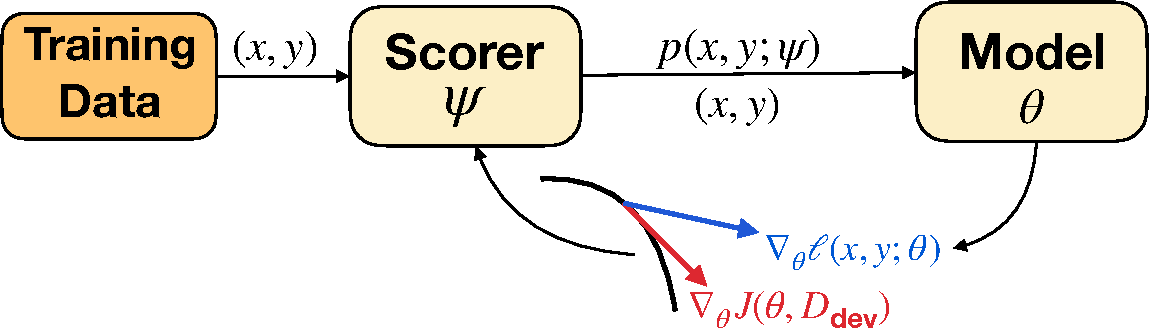
\includegraphics[width=0.5\textwidth]{figs/method_plot_crop.pdf}
    \caption{The general workflow of \dds.}
    \label{fig:method}
\end{figure}

In this section, we provide an intuitive explanation of how we update the model parameter $\theta$ and its adaptive weighting parameter $\psi$. Given the current optimal $\psi_t$ at time $t$, we can update $\theta$ as
\begin{align}
    \label{eqn:theta_update}
    \theta_t \leftarrow \theta_{t-1} + \alpha \nabla_\theta J(\theta_{t-1}, \psi_t)
\end{align}
where $\alpha$ is the learning rate for the model parameter $\theta$. The key problem left is, how can we optimize $\psi$ so that it provides the up-to-date data importance weights for the model $\theta_t$ at any time $t$ during training?

A straight-forward optimization strategy for $\psi$ is through Reinforcement Learning~(RL). Figure \ref{fig:method} illustrates the general framework of our method, where we can formulate the basic RL components as: the \textbf{agent} to optimize is the scorer, or data weighting function $P(x, y; \psi)$; the \textbf{state} is the current model parameter $\theta$; the \textbf{reward} $R(x, y)$ is the change in dev set risk $\Delta J_{\text{dev}}(x, y) = J(\theta_t, \mathcal{D}_\text{dev}) - J(\theta_{t-1}, \mathcal{D}_\text{dev})$, where $\theta_t$ is the new model parameter after updating $\theta_{t-1}$ using the training data $(x, y)$.

However, the above RL framework is difficult to implement in practice because of the drastic variance and credit assignment trade off in the reward function $\Delta J_{\text{dev}}(x, y)$: if we want to get clear credit assignment of a single training data pair $(x, y)$, its reward $\Delta J_{\text{dev}}(x, y)$ would be very noisy; to reduce the variance in $\Delta J_{\text{dev}}(x, y)$, we need a large number of training pairs $(x, y) = \{(x_0, y_0), (x_1, y_1), ..., (x_i, y_i)\}$. These examples would all get assigned the same amount of reward, while ideally they might have different level of influence on the final model performance.

To address this difficulty, we propose a novel reward function as an approximation to $\Delta J_{\text{dev}}(x, y)$ to quantify the effect of the training data $(x, y)$. In general, we prefer data that moves $\theta$ in the direction that minimizes the dev set risk. Therefore, we can use the agreement between the model gradient on data $(x, y)$ and the gradient on the dev set to approximate the \textit{change} in dev set risk brought by $(x, y)$. That is, 
\begin{align}
    \label{eqn:reward_fn}
    R(x, y) = \Delta J_{\text{dev}}(x, y) \approx \nabla_\theta \ell(x, y; \theta_{t-1}) \cdot \nabla_\theta J(\theta_t, \mathcal{D}_\text{dev}) 
\end{align}

According to the REINFORCE algorithm, the update rule for $\psi$ is thus
\begin{align}
    \label{eqn:psi_update}
    \psi_{t+1} \leftarrow  \psi_t + \eta \underbrace{\nabla_\theta \ell(x, y; \theta_{t-1}) \cdot \nabla_\theta J(\theta_t, \mathcal{D}_\text{dev})}_{\mathclap{R(x, y)}} \nabla_\psi \text{log}(P(X, Y;\psi))
\end{align}
where $\eta$ is the learning rate for the data importance parameter $\psi$. As shown in Figure \ref{fig:method}, by alternating between Eqn. \ref{eqn:theta_update} and Eqn. \ref{eqn:psi_update}, we can iteratively update $\theta$ using the adaptively weighted training data, and update $\psi$ to optimize data weighting for $\theta$. Now that we explain the intuition behind our method, we provide the mathematical derivation of the update rules in the next section.  

\subsection{\label{sec:diff_data_selection}Direct Differentiation}

The connection between $\psi$ and $\theta$ in Eqn. \ref{eqn:psi_theta_argmin} shows that $J(\theta_t, \mathcal{D}_\text{dev})$ is differentiable with respect to $\psi$. Notably, it is a specific case of bi-level optimization~\citep{bilevel_optim}, which has been applied to works on optimization~\citep{hyper_grad}, meta-learning~\citep{finn2017model}, and neural architecture search~\citep{darts}. To our knowledge, we are the first to utilize bi-level optimization for data selection. 

By the chain rule, we can compute the gradient $\nabla_\psi J(\theta_t, \mathcal{D}_\text{dev})$ as follows:
\begin{equation}
  \label{eqn:two_step_update}
   \small
  \begin{aligned}
    \nabla_\psi J(\theta_t, \mathcal{D}_\text{dev})
      &= \nabla_{\theta_t} J(\theta_t, \mathcal{D}_\text{dev})^\top \cdot \nabla_\psi \theta_t(\psi) &\text{(chain rule)} \\
      &= \nabla_{\theta_t} J(\theta_t, \mathcal{D}_\text{dev})^\top \cdot \nabla_\psi \left( \theta_{t-1} - \nabla_\theta J(\theta_{t-1}, \psi) \right) &\text{(substitute $\theta_t$ from Eqn~\ref{eqn:theta_update})} \\
      &\approx -\nabla_{\theta_t} J(\theta_t, \mathcal{D}_\text{dev})^\top \cdot \nabla_\psi  \left( \nabla_\theta J(\theta_{t-1}, \psi) \right) &\text{(assume $\nabla_\psi \theta_{t-1} \approx 0$)} \\
      &= \nabla_\psi \mathbb{E}_{x, y \sim p(X, Y; \psi)} \left[J(\theta_t, \mathcal{D}_\text{dev})^\top \cdot \nabla_\theta \ell(x, y; \theta_{t-1} )\right] \\
    &= \mathbb{E}_{x, y \sim p(X, Y; \psi)} \left[\left( J(\theta_t, \mathcal{D}_\text{dev})^\top \cdot \nabla_\theta \ell(x, y; \theta_{t-1} ) \right) \cdot \nabla_\psi \log{p(x, y; \psi)} \right]
  \end{aligned}
\end{equation}
Here, we make a Markov assumption that $\nabla_\psi \theta_{t-1} \approx 0$, assuming that at step $t$, given $\theta_{t-1}$ we do not care about how the values of $\psi$ from previous steps led to $\theta_{t-1}$. Eqn~\ref{eqn:two_step_update} leads to a rule to update $\psi$ using gradient descent:
\begin{equation}
  \label{eqn:psi_update_rule}
   \small
  \begin{aligned}
    \psi_{t+1} 
      &\leftarrow \psi_t + \eta \left( J(\theta_t, \mathcal{D}_\text{dev})^\top \cdot \nabla_\theta \ell(x, y; \theta_{t-1} ) \right) \cdot \nabla_\psi \log{p(x, y; \psi)},
  \end{aligned}
\end{equation}
where $\eta$ is the learning rate for $\psi$, which is a hyper-parameter. Now we can see that our derived update rule Eqn. \ref{eqn:psi_update_rule} matches the RL update rule according to our proposed reward function in Eqn. \ref{eqn:psi_update}. Since our formulation allows direct differentiation to optimize $\psi$, we name it Differentiable Adaptive Weighting~(\dds).

The connection between our design of the reward function and the direct derivation of the gradient of $\psi$ raises a potential concern with our approach: because we optimize $\psi_t$ directly on the dev set using $J(\theta_t, \mathcal{D}_\text{dev})$, we may risk indirectly overfitting model parameters $\theta_t$ by selecting a small subset of data that is overly specialized.
However we do not observe this problem in practice, and posit that this because (1) the influence of $\psi_t$ on the final model parameters $\theta_t$ is quite indirect, and acts as a ``bottleneck'' which has similarly proven useful for preventing overfitting in neural models \cite{grezl2007probabilistic}, and (2) because the actual implementations of DDS~(which we further discuss in Section \ref{sec:formualtion}) only samples a subset of data from $\mathcal{D}_\text{train}$ at each optimization step, further limiting expressivity.


\dds~operates by alternating Eqn~\ref{eqn:theta_update} and Eqn~\ref{eqn:psi_update} on batches of training data and dev data respectively. To implement Eqn~\ref{eqn:psi_update_rule} we need two approximations.
First, in practice the size of $\mathcal{D}_\text{train}$ is usually too large for exact calculation of the gradient $\nabla_\theta$. To overcome this difficulty, we adopt an importance sampling strategy, which can be implemented in two ways:
(1) We can sample a subset of $\mathcal{D}_{\text{train}}$ with a uniform proposal distribution $\hat{x}, \hat{y} \sim \text{Uniform}(\mathcal{D}_\text{train})$, then scale the probabilities in Eqn~\ref{eqn:psi_theta_argmin} by $p(\hat{x}, \hat{y}; \psi)$ over only this subset of data.
(2) We can similarly sample a subset of $\mathcal{D}_{\text{train}}$ uniformly, but then take a Monte-Carlo estimate of this quantity by further sub-sampling the data according to $p(\hat{x}, \hat{y}; \psi)$.
Second, the exact gradient for $\psi$ depends on the optimization algorithm that we use for $\theta$, and we discuss some concrete formulations in Appendix \ref{app:grad_of_optimizers}.
\section{\label{sec:formualtion}Concrete Instantiations of DDS}

%\gn{I made a few changes here, please tell me if you think they aren't warranted: (1) I moved this sentence into this section from the end of the previous section, (2) I removed the mention of ``Momentum'' and ``Adam'' in the below sentence, as it seemed to hurt generality, (3) I tried to note that image classification is ``generic'' and multilingual NMT is ``specific'', so as a general ML paper people can see that this is both broadly applicable and customizable.}
We now turn to discuss two concrete instantiations of DDS that we use in our experiments: a more generic example of classification, which should be applicable to a wide variety of tasks, and a specialized application to the task of multilingual NMT, which should serve as an example of how DDS can be adapted to the needs of specific applications.

%\gn{In the following, for further generality, (1) can we turn ``Image Classification'' into just ``Classification''? (2) can we remove any other details that hurt the generality of the approach such as specific mention of ``Momentum'' or ``Adam'', mentioning that the classification model is a CNN, etc.? These can be moved to the experiments.}

\subsection{\label{sec:image_method}Formulation for Classification}

%\begin{wraptable}{l}{8cm}
    \vspace{-0.2cm}
\begin{center}
\resizebox{!}{3cm}{
\begin{algorithm}[H]
\SetAlgoLined
\DontPrintSemicolon
\SetKwInOut{Input}{Input}
\SetKwInOut{Output}{Output}
\SetCommentSty{itshape}
\SetKwComment{Comment}{$\triangleright$\ }{}
\Input{$\mathcal{D}_\text{train}$, $\mathcal{D}_\text{dev}$}
\Output{Optimal parameters $\theta^*$}
 Initializer $\theta_0$ and $\psi_0$
 
 \For{$t = 1$~\textbf{\emph{to}}~$\text{num\_train\_steps}$}{
    Sample $B$ training data points $x_i, y_i \sim \text{Uniform}(\mathcal{D}_\text{train})$
    
    Sample $B$ validation data points $x'_i, y'_i \sim \text{Uniform}(\mathcal{D}_\text{dev})$
  
    \Comment{Train $\theta$ for one step}
    Update $\theta_t \leftarrow \text{GradientUpdate}\Big(\theta_{t-1}, \sum_{i=1}^{B} p(x_i, y_i; \psi_{t-1}) \nabla_\theta \ell(x_i, y_i; \theta_{t-1}) \Big)$
    \label{alg:grad_update_model}
    
    \Comment{Evaluate $\theta_t$ on $\mathcal{D}_\text{dev}$}
    Let $d_\theta \leftarrow \frac{1}{B} \sum_{j=1}^{B} \nabla_\theta \ell(x'_j, y'_j; \theta_t)$
  
    \Comment{Compute gradient of $\psi$}
    Let $d_\psi \leftarrow \frac{1}{B} \sum_{i=1}^{B} \left[ \Big( d_\theta^\top \cdot \nabla_\theta \ell(x_i, y_i; \theta_{t-1}) \Big) \cdot \nabla_\psi \log{p(x_i, y_i; \psi)} \right]$
    \label{alg:require_per_example_grad}
    
    Update $\psi_t \leftarrow \text{GradientUpdate}(\psi_{t-1}, d_\psi)$
    \label{alg:grad_update_p}
  }
  \caption{\label{alg:image_classification_dds}Training a classification model with DDS.}
\end{algorithm}
}
\end{center}
    \vspace{-0.2cm}

%\end{wraptable}
Algorithm~\ref{alg:image_classification_dds} presents the pseudo code for the training process on classification tasks, using the notations introduced in Section~\ref{sec:method}. 
The main  classification model is parameterized by $\theta$. The \dds~model $p(X, Y; \psi)$ is an identical network with the main model, but with independent weights, \ie~$p(X, Y; \psi)$ does not share weights with $\theta$. For each example $x_i$ in a minibatch uniformly sampled from $\mathcal{D}_\text{train}$, this \dds~model outputs a scalar from the data $x_i$. All scalars are passed through a softmax function to compute the relative probabilities of the examples in the minibatch, and their gradients are scaled accordingly when applied to $\theta$. Note that our actual formulation of $p(X, Y; \psi)$ does \textit{not} depend on $Y$, but we keep $Y$ in the notation for consistency with the formulation of the \dds~framework. Note that we have two gradient update steps, one for the model parameter $\theta_t$ in Line~\ref{alg:grad_update_model} and the other for the DDS parameter $\psi$ in Line~\ref{alg:grad_update_p}. For the model parameter update, we can simply use any of the standard optimization update rule. For the DDS parameter $\psi$, we use the update rule derived in Section \ref{sec:grad_of_optimizers}.

\paragraph{Per-Example Gradient.} As seen from Line~\ref{alg:require_per_example_grad} of Algorithm~\ref{alg:image_classification_dds}, as well as from Eqn~\ref{eqn:momentum_update_for_psi}, \dds~requires us to compute $\nabla_\theta \ell(x_i, y_i; \theta_{t-1})$, \ie~the gradient for each example in a batch of training data. This operation is very slow and memory intensive, especially when the batch size is large, \eg~our experiments on ImageNet use a batch size of $4096$ (see~Section~\ref{sec:experiment}). Therefore, we propose an efficient approximation of this per-example gradient computation via the first-order Taylor expansion of $\ell(x_i, y_i; \theta_{t-1})$. In particular, for any vector $v \in \mathbb{R}^{\ABS{\theta}}$, with sufficiently small $\epsilon > 0$, we have:
    \vspace{-0.15cm}
\begin{equation}
  \label{eqn:taylor_dot_product}
  \small
  \begin{aligned}
    v^\top \cdot \nabla_\theta \ell(x_i, y_i; \theta_{t-1})
    \approx
    \frac{1}{\epsilon}
    \left(
      \ell\big( x_i, y_i; \theta_{t-1} + \epsilon v \big) -
      \ell\big( x_i, y_i; \theta_{t-1} \big)
    \right),
  \end{aligned}
\end{equation}
    %\vspace{-0.1cm}
Eqn~\ref{eqn:taylor_dot_product} can be implemented by keeping a shadow version of parameters $\theta_{t-1}$, caching training loss $\ell(x_i, y_i; \theta_{t-1})$, and computing the new loss with $\theta_{t-1} + \epsilon v$. Here, $v$ is $d_\theta$ as in Line~\ref{alg:require_per_example_grad} of Algorithm~\ref{alg:image_classification_dds}.

\subsection{\label{sec:nmt_method}Formulation for Multilingual NMT}

Next we demonstrate an application of \dds~to multilingual models for NMT, specifically for improving accuracy on low-resource languages (LRL)~\citep{nmt_transfer,rapid_adapt_nmt}.

In this setting, we assume that we have a particular LRL $S$ that we would like to translate into target language $T$, and we additionally have a multilingual corpus $\mathcal{D}_{\text{train}}$ that has parallel data between $n$ source languages $(S_1, S_2, ..., S_n)$ and target language $T$. We would like to pick parallel data from any of the source languages to the target language to improve translation of a particular LRL $S$, so we assume that $\mathcal{D}_{\text{dev}}$ exclusively consists of parallel data between $S$ and $T$.
Thus, \dds~will select data from $\mathcal{D}_{\text{train}}$ that improve accuracy on $S$-to-$T$ translation as represented by $\mathcal{D}_{\text{dev}}$.

To make training more efficient and stable in this setting, we make three simple modifications of the main framework in Section \ref{sec:diff_data_selection} that take advantage of the problem structure of multilingual NMT.
First, instead of directly modeling $p(X,Y;\psi)$, we assume a uniform distribution over the target sentence $Y$, %($p(Y)$)
and only parameterize the conditional distribution of which source language sentence to pick given the target sentence: $p(X|y;\psi)$. This design follows the formulation of Target Conditioned Sampling~(TCS;~\citet{TCS}), an existing state-of-the-art data selection method that uses a similar setting but models the distribution $p(X|y)$ using heuristics.  Since the scorer only needs to model a simple distribution over training languages, we use a fully connected 2-layer perceptron network.
Second, we only update $\psi$ after updating the NMT model for a fixed number of steps.
Third, we sample the data according to $p(X|y;\psi)$ to get a Monte Carlo estimate of the objective in Eqn.~\ref{eqn:psi_theta_argmin}.
This significantly reduces the training time compared to using all data.
The pseudo code of the training process is in Algorithm~\ref{alg:nmt_dds}.

% We then train a parameterized distribution $p(x, y;\psi)$ with a support over $\mathcal{D}_{\text{train}}$, such that selecting training data according to this distribution leads to the optimal NMT model $\theta^*$ on the language $S$. 
%That is, $\psi$ satisfies the following condition
%\begin{equation}
%  \label{eqn:nmt_argmin}
%  \begin{aligned}
%    \arg\min_\psi
%    \sum_{x_i, y_i \in S\text{-}Y} \ell_{\text{dev}}(x_i, y_i; \theta^*)
%    ~~~\text{where}~~~
%    \theta^* = \arg\min_\theta \mathbb{E}_{x_i,y_i \sim p(X, Y;\psi)}\left[ \ell_{\text{train}}(x_i, y_i; \theta) \right]
%  \end{aligned}
%\end{equation}
%\begin{wraptable}{l}{8cm}
    %\vspace{-0.3cm}

%\begin{center}
\resizebox{!}{0.6\columnwidth}{
\begin{algorithm}[H]
\SetAlgoLined
\DontPrintSemicolon
\SetKwInOut{Input}{Input}
\SetKwInOut{Output}{Output}
\SetCommentSty{itshape}
\SetKwComment{Comment}{$\triangleright$\ }{}
%\KwResult{Write here the result }

\Input{$\mathcal{D}_{\text{train}}$; K: number of data to train the NMT model before updating $\psi$; 
E: number of updates for $\psi$; 
$\alpha_1$,$\alpha_2$: discount factors for the gradient}
%}
\Output{The converged NMT model $\theta^*$}

  Initialize $\psi_0$, $\theta_0$
  
  \Comment{Initialize the gradient of each source language}
  $grad[S_i] \leftarrow 0$ \textbf{for} \textit{i in n}
  %\For{ i in n}{
  %
  %  $grad[S_i] \leftarrow 0$
  %  
  %}
 
  \While{$\theta$ not converged}{
    %\Comment{Sample training data according to $\psi$}
    $X, Y \leftarrow \text{load\_data}(\psi, \mathcal{D}_{\text{train}}, K)$  \label{alg:load_nmt}
  
    \Comment{Train the NMT model}
    \For{ $x_i, y$ in $X, Y$}{
      $\theta_t \leftarrow \text{GradientUpdate}\left( \theta_{t-1}, \nabla_{\theta_{t-1}} \ell(x_i, y; \theta_{t-1}) \right)$
        
      $grad[S_i] \leftarrow \alpha_1 \times \text{grad}[S_i] + \alpha_2 \times \nabla_{\theta_{t-1}} \ell(x_i, y; \theta_{t-1})$
    }
    %\Comment{Compute gradient for all languages}
   %\For{ $i$ from $1$ to $n$}{
        
    %Sample $B$  data points $x_i, y_i$ from language $S_i$
    
      %$grad[S_i] \leftarrow  \nabla_{\theta} \ell(x_i, y; \theta)$
    %}
    \Comment{Optimize $\psi$}
    \For{ iter in E}{
      
      sample $B$ data pairs from $\mathcal{D}_{\text{train}}$
      
      $d_\psi \leftarrow \frac{1}{B} \sum_{j=1}^B \sum_{i=1}^n  \Big[ & \text{grad}[S_i]^\top \text{grad}[S]  \\
      \quad\quad\quad\quad \cdot \nabla_{\psi_{t-1}} \text{log}\left( p\left( S_i|y_j;\psi_{t-1} \right) \right) \Big]$
       
      $\psi_t \leftarrow \text{GradientUpdate}(\psi_{t-1}, d_{\psi_{t-1}})$ 
    }
  }
  \caption{\label{alg:nmt_dds}Training multilingual NMT with \dds.}
\end{algorithm}
}
%\end{center}

%\end{wraptable} 


%Note that in Line \ref{alg:load_nmt} of Algorithm \ref{alg:nmt_dds}, we load $K$ training data according to $p(\psi)$. Since we formulate $p(\psi)$ as $p(S_i|y;\psi)$, the data loading procedure is the same as the TCS algorithm~\citep{TCS}: for each of the $K$ target sentences, we calculate a distribution over its source languages according to $p(S_i|y;\psi)$, and then sample the corresponding source sentences based on this distribution.

 


\begin{table*}[t]
  \caption{\label{tab:results}Results for image classification accuracy (left) and multilingual MT BLEU (right). For MT, the statistical significance is indicated with $*$ (p $<$ 0.005) and $\dagger$ (p $<$ 0.0001). \dds~ outperforms the best baseline in all settings. }
  \vspace{0.2cm}
   \begin{minipage}{.575\linewidth}
    \resizebox{\textwidth}{!}{
      \begin{tabular}{lcccc}
        \toprule
        \multirow{2}{*}{\textbf{Methods}}
        & \multicolumn{2}{c}{CIFAR-10 (WRN-28-$k$)} & \multicolumn{2}{c}{ImageNet (ResNet-50)} \\
        \cmidrule(lr){2-3} \cmidrule(lr){4-5}
        & 4K, $k=2$ & Full, $k=10$ & 10\% & Full \\
        \midrule
        Uniform &
        82.60$\pm$0.17 &
        95.55$\pm$0.15 & 
        56.36/79.45 &
        76.51/93.20 \\
        SPCL &
        81.09$\pm$0.22 &
        93.66$\pm$0.12 & 
        - &
        - \\
        BatchWeight &
        79.61$\pm$0.50 &
        94.11$\pm$0.18 & 
        - &
        - \\
        MentorNet &
        83.11$\pm$0.62 &
        94.92$\pm$0.34 & 
        - &
        - \\
        \midrule
        \dds     &
        83.63$\pm$ 0.29 &
        96.31$\pm$ 0.13 &
        \textbf{56.81}/\textbf{79.51} &
        \textbf{77.23}/\textbf{93.57} \\
         retrained \dds     &
        \textbf{85.56}$\pm$\textbf{0.20} &
        \textbf{97.91}$\pm$\textbf{0.12} &
        - &
        - \\       
        \bottomrule
      \end{tabular}
      }
      \end{minipage}
  \begin{minipage}{.42\linewidth}
    \resizebox{\textwidth}{!}{
      \begin{tabular}{l|cccc}
        \toprule
        \textbf{Methods} & \textbf{aze} & \textbf{bel} & \textbf{glg} & \textbf{slk} \\
        \midrule
        Uniform & 10.31 & 17.21 & 26.05 & 27.44 \\
        SPCL & 9.07 & 16.99 & 23.64 & 21.44 \\
        Related & 10.34 & 15.31 & 27.41 & 25.92 \\
        TCS     & 11.18 & 16.97 & 27.28 & 27.72 \\
        \midrule
        \dds     & 10.74 & 17.24 & 27.32 & $\mathbf{28.20^*}$ \\
        TCS+\dds & $\mathbf{11.84^*}$ & $\mathbf{17.74^\dagger}$ & \textbf{27.78} & 27.74 \\
        \bottomrule
      \end{tabular}
      }
      \end{minipage}
\end{table*}

\section{\label{sec:experiment}Experiments}
%\gn{You need at least one sentence of lead-in here.}
We now discuss experimental results on both image classification, an instance of the general classification problem using Algorithm \ref{alg:image_classification_dds}, and multilingual NMT using Algorithm \ref{alg:nmt_dds}.

\subsection{\label{exp:settings}Experimental Settings}

\noindent \textbf{Data.} We apply our method on established benchmarks for image classification and multilingual NMT.
For image classification, we use CIFAR-10~\citep{cifar10} and ImageNet~\citep{imagenet}. For each dataset, we consider two settings: a reduced setting where only roughly 10\% of the training labels are used, and a full setting, where all labels are used. Specifically, the reduced setting for CIFAR-10 uses the first $4000$ examples in the training set, and with ImageNet, the reduced setting uses the first $102$ TFRecord shards as pre-processed by~\citet{imagenet_generalize_better}. We use the size of $224 \times 224$ for ImageNet.

For multilingual NMT, we use the 58-language-to-English TED dataset~\citep{ted_pretrain_emb}. 
Following prior work~\citep{ted_pretrain_emb,rapid_adapt_nmt,sde}, we evaluate translation from four low-resource languages~(LRL) Azerbaijani~(\texttt{aze}), Belarusian~(\texttt{bel}), Galician~(\texttt{glg}), and Slovak~(\texttt{slk}) to English, where each is paired with a similar high-resource language Turkish~(\texttt{tur}), Russian~(\texttt{rus}), Portugese~(\texttt{por}), and Czech~(\texttt{ces}) (details in Appendix~\ref{app:nmt_data}).
We combine data from all 8 languages, and use \dds~to optimize data selection for each LRL. 

\noindent \textbf{Models and Training Details.}
For image classification, on CIFAR-10, we use the pre-activation WideResNet-28~\citep{wide_res_net}, with width factor $k=2$ for the reduced setting and $k=10$ for the normal setting. For ImageNet, we use the post-activation ResNet-50~\citep{res_net}. 
%The batch sizes for CIFAR-10 and for ImageNet are $128$ and $4096$, running for 200K steps and 40K steps, respectively. 
%We use the standard Momentum update for the \dds~model parameter $\theta$, and the derived Momentum update rule in Section~\ref{sec:grad_of_optimizers} for the \dds~distribution parameter $\psi$, both with the momentum rate of $0.9$.
These implementations reproduce the numbers reported in the literature~\citep{wide_res_net,res_net,resnext}, and additional details can be found in Appendix \ref{app:image_hparam}.

For NMT, we use a standard LSTM-based attentional baseline \citep{attention}, which is similar to previous models used in low-resource scenarios both on this dataset~\citep{rapid_adapt_nmt,sde} and others~\citep{lownmt19} due to its relative stability compared to other options such as the Transformer \citep{vaswani2017attention}. Accuracy is measured using BLEU score \citep{bleu}.
More experiment details are noted in Appendix \ref{app:nmt_hparam}.

\noindent \textbf{Baselines and Our Methods.}
For both image classification and multi-lingual NMT, we compare the following data selection methods.
\begin{itemize}
\item \textbf{Uniform}: data is selected uniformly from all of the data that we have available, as is standard in training models. 
\item \textbf{SPCL}~\citep{spcl}: a curriculum learning method that dynamically updates the curriculum to focus more on the ``easy'' training examples based on model loss.
\item \textbf{\dds}: our proposed method.
\end{itemize}

For image classification, we compare with several additional methods designed for filtering noisy data on CIFAR-10, where we simply consider the dev set as the clean data.
\begin{itemize}
\item \textbf{BatchWeight}~\citep{learn_reweight}: a method that scales example training loss in a batch with a locally optimized weight vector using a small set of clean data. 
\item  \textbf{MentorNet}~\citep{mentornet}: a curriculum learning method that trains a mentor network to select clean data based on features from both the data and the main model. 
\end{itemize}


For machine translation, we also compare with two state-of-the-art heuristic methods for multi-lingual data selection.
\begin{itemize}
\item \textbf{Related}: data is selected uniformly from the target LRL and a linguistically related HRL \citep{rapid_adapt_nmt}. 
\item  \textbf{TCS}: a recently proposed method of ``target conditioned sampling'', which uniformly chooses target sentences, then picks which source sentence to use based on heuristics such as word overlap \citep{TCS}.
Note that both of these methods take advantage of structural properties of the multi-lingual NMT problem, and do not generalize to other problems such as classification.
\end{itemize}

%\gn{This is a little bit sudden to appear here directly in the experiments section. It might be good to mention this at the end of Section \ref{sec:efficient_reward} as a method to incorporate prior information? I think mentioning this there is actually a very good thing, as it adds to another thing that the proposed framework can do. If we mention it here, on the other hand, it seems a little bit like a hack that we added on at the last minute to make things work.}
\paragraph{DDS with Prior Knowledge} \dds~is a flexible framework to incorporate prior knowledge about the data using the scorer network, which can be especially important when the data has certain structural properties such as language or domain. We test such a setting of \dds~for both tasks.

For image classification, we use \textbf{retrained \dds}, where we first train a model and scorer network using the standard \dds~till convergence. The trained scorer network can be considered as a good prior over the data, so we use it to train the final model from scratch again using \dds. For multilingual NMT, we experiment with \textbf{TCS+\dds}, where we initialize the parameters of \dds~with the TCS heuristic, then continue training. 



% \noindent \textbf{Data Selection Baselines.} We compare our method against three strong baselines: 1) All: all 8 languages are used for training without any data selection; 2) Bi: we train on the combined datasets of each LRL and its related HRL, which is a special case of data selection that requires prior linguistic knowledge; 3) TCS~\citep{TCS}: the state-of-the-art data selection method for multilingual NMT. Given a target sentence, TCS conditionally samples a source sentence from the candidate languages based on simple heuristics such as vocabulary overlap.

%\gn{Just a comment: I'm not a huge fan of this because it seems a bit hacky, but if it's what was necessary to make things work this time then that's fair}. 
% We note that all these three tricks are not needed for our experiments on CIFAR-10, where the batch size is much smaller.

\subsection{Main Results}


%\begin{table}[t]
%  \captionof{table}{\label{tab:results}Results for image classification accuracy (left) and multilingual MT BLEU (right). For MT, the statistical significance is indicated with $*$ (p < 0.005) and $\dagger$ (p < 0.0001).}
%  \begin{minipage}{.575\linewidth}
%    \resizebox{\textwidth}{!}{
%      \begin{tabular}{lcccc}
%        \toprule
%        \multirow{2}{*}{\textbf{Methods}}
%        & \multicolumn{2}{c}{CIFAR-10 (WRN-28-$k$)} & \multicolumn{2}{c}{ImageNet (ResNet-50)} \\
%        \cmidrule(lr){2-3} \cmidrule(lr){4-5}
%        & 4K, $k=2$ & Full, $k=10$ & 10\% & Full \\
%        \midrule
%        Uniform &
%        82.60$\pm$0.17 &
%        95.55$\pm$0.15 & 
%        56.36/79.45 &
%        76.51/93.20 \\
%        SPCL &
%        81.09$\pm$0.22 &
%        93.66$\pm$0.12 & 
%        - &
%        - \\
%        BatchWeight &
%        79.61$\pm$0.50 &
%        94.11$\pm$0.18 & 
%        - &
%        - \\
%        MentorNet &
%        83.11$\pm$0.62 &
%        94.92$\pm$0.34 & 
%        - &
%        - \\
%        \midrule
%        \dds     &
%        83.63$\pm$ 0.29 &
%        96.31$\pm$ 0.13 &
%        \textbf{56.81}/\textbf{79.51} &
%        \textbf{77.23}/\textbf{93.57} \\
%         retrained \dds     &
%        \textbf{85.56}$\pm$\textbf{0.20} &
%        \textbf{97.91}$\pm$\textbf{0.12} &
%        - &
%        - \\       
%        \bottomrule
%      \end{tabular}
%    }
%  \end{minipage}
%  \begin{minipage}{.425\linewidth}
%    \resizebox{\textwidth}{!}{
%      \begin{tabular}{l|cccc}
%        \toprule
%        \textbf{Methods} & \textbf{aze} & \textbf{bel} & \textbf{glg} & \textbf{slk} \\
%        \midrule
%        Uniform & 10.31 & 17.21 & 26.05 & 27.44 \\
%        SPCL & 9.07 & 16.99 & 23.64 & 21.44 \\
%        Related & 10.34 & 15.31 & 27.41 & 25.92 \\
%        TCS     & 11.18 & 16.97 & 27.28 & 27.72 \\
%        \midrule
%        \dds     & 10.74 & 17.24 & 27.32 & $\mathbf{28.20^*}$ \\
%        TCS+\dds & $\mathbf{11.84^*}$ & $\mathbf{17.74^\dagger}$ & \textbf{27.78} & 27.74 \\
%        \bottomrule
%      \end{tabular}
%    }
%  \end{minipage}
%  \vspace{-4mm}
%\end{table}

% \begin{wraptable}{r}{0.6\textwidth}
% %\begin{adjustbox}{max width=0.7\textwidth}
% \vspace{-1cm}
% \resizebox{0.6\textwidth}{!}{
%   \begin{tabular}{llll}
%     \multicolumn{4}{c}{\textbf{CIFAR-10} ($\text{mean} \pm \text{std}$ over $10$ runs)} \\
%   \toprule
%     \textbf{Portion} &
%     \textbf{Model} &
%     \textbf{Baseline} &
%     \textbf{\\dds}
%     \\
%   \midrule
%     4K &
%     WideResNet-28-2 &
%     $82.60 \pm 0.17$ & % 6109331
%     $\mathbf{83.63 \pm 0.29}$ % 6109486
%     \\
%     Full &
%     WideResNet-28-10 &
%     $95.55 \pm 0.15$ &  % 6153155
%     $\mathbf{96.31 \pm 0.13}$  % 6170380
%     \\
%   \bottomrule
%     \\
%     \multicolumn{4}{c}{\textbf{ImageNet} ($\text{Top-1}/\text{Top-5}$)} \\
%     \toprule
%     \textbf{Portion} &
%     \textbf{Model} &
%     \textbf{Baseline} &
%     \textbf{\\dds}
%     \\
%   \midrule
%     10\%  & ResNet-50 &
%     $56.36 / 79.45$ & % 5267621/workUnits/118
%     $\mathbf{56.81 / 79.51}$   % 6020481/workUnits/18
%     \\  
%     Full & ResNet-50 &
%     $76.51 / 93.20$ & % https://arxiv.org/abs/1810.12890
%     $\mathbf{77.23 / 93.57}$ % 6800564/workUnits/39
%     \\
%     \bottomrule
%   \end{tabular}
% }
%   \captionof{table}{\label{tab:image_classification_results}Image classification accuracy. Higher is better.}
% %\end{adjustbox}
% %\end{center}
% \end{wraptable}

% \noindent \textbf{Results.} Results are presented in Table~\ref{tab:image_classification_results}. As can be seen, \\dds~improves the performance of all tasks considered. The best improvement is for CIFAR-10 using 4K labels. We posit that this is because when the  
%\gn{The following explanation is pretty weak because increasing the degrees of freedom of the model was not even one of our original motivations. Is there any way we can at least say something about how it (might be?) reducing the weight on outliers or something like that?} In our intuitions, \\dds~provides an extra degree of freedom to train the models, namely the per-example scaling of gradients. This extra degree of freedom is well-utilized by the $p(\hat{x}, \hat{y}; \psi)$ distribution, leading to the improvements.


% \subsection{Multilingual NMT}
% 
% \noindent \textbf{Baselines.} We compare our method against three strong baselines: 1) All: all 8 languages are used for training without any data selection; 2) Bi: we train on the combined datasets of each LRL and its related HRL, which is a special case of data selection that requires prior linguistic knowledge; 3) TCS~\citep{TCS}: the state-of-the-art data selection method for multilingual NMT. Given a target sentence, TCS conditionally samples a source sentence from the candidate languages based on simple heuristics such as vocabulary overlap.
% 
% \noindent \textbf{Implementation.} Here we clarify several design choices for Algorithm \ref{alg:nmt_\dds}. To model the distribution $p(S_i|y;\psi)$, we use a 2-layer feed-forward network with hidden size of 32. The input vector for the network is a vector of size of source languages $n$, representing which of the languages contain a corresponding source sentence for a given target sentence $y$. We use the standard Adam update rule with learning rate of 0.001 for the NMT model parameter $\theta$, and the derived Adam update rule from Section~\ref{sec:grad_of_optimizers} with learning rate~0.0001 for the distribution parameter $\psi$. 
% 
% We test two different settings for using \dds for multilingual  NMT: 1) TCS+\dds: we pretrain the network with the heuristic distribution from TCS before the \dds training process
% %. K in Algorithm \ref{alg:nmt_dds} is set to be 50,000; 
% 2) Uniform+DDS: we train the network for $\psi$ from scratch. %At the start of training, K is set to be 5,000 to encourage exploration; after updating $\psi$ for 5 times, we also set it to 50,000.
% We run all experiments with 3 different random seeds and pick the median for each method. Additional hyperparameters are listed in Appendix~\ref{app:nmt_hparam}.
% 
% \noindent \textbf{Results.}
% \begin{wraptable}{l}{0.6\textwidth}
% \begin{center}
% \vspace{-0.5cm}
%     \begin{tabular}{l|cccc}
%     \toprule
%     \textbf{Model} & \textbf{aze} & \textbf{bel} & \textbf{glg} & \textbf{slk} \\
%     \midrule
%     All & 10.31 & 17.21 & 26.05 & 27.44 \\
%     Bi & 10.34 & 15.31 & 27.41 & 25.92 \\
%     TCS & 11.18 & 16.97 & 27.28 & 27.72 \\
%     \midrule
%     TCS+DDS & \textbf{11.84} & \textbf{17.74} & \textbf{27.78} & 27.74 \\
%     %Uniform & 9.54 & 14.75 & 25.11 & 26.30 \\
%     Uniform+DDS & 10.74 & 17.24 & 27.32 & \textbf{28.20} \\
%     \bottomrule
%     \end{tabular}
%      \captionof{table}{\label{tab:nmt_result}BLEU score. Higher is better.}
% \end{center}
% \vspace{-0.5cm}
% \end{wraptable}

The results of the baselines and our method are listed in Table \ref{tab:results}.
First, comparing the standard baseline strategy of ``Uniform'' and the proposed method of ``\dds'' we can see that in all 8 settings \dds~improves over the uniform baseline. This is a strong indication of both the consistency of the improvements that \dds~can provide, and the generality -- it works well in two very different settings. Next, we find that \dds~outperforms SPCL by a large margin for both of the tasks, especially for multilingual NMT. This is probably because SPCL weighs the data only by their easiness, while ignoring their relevance to the dev set, which is especially important in settings where the data in the training set can have very different properties such as the different languages in multilingual NMT. 

\dds~also brings improvements over the state-of-the-art intelligent data utilization methods. For image classification, \dds~outperforms MentorNet and BatchWeight on CIFAR-10 in all settings. For NMT, in comparison to Related and TCS, vanilla \dds~performs favorably with respect to these state-of-the-art data selection baselines, outperforming each in 3 out of the 4 settings (with exceptions of slightly underperforming Related on \texttt{glg} and TCS on \texttt{aze}).
In addition, we see that incorporating prior knowledge into the scorer network leads to further improvements. For image classification, retrained \dds~can significantly improve over regular \dds, leading to the new state-of-the-art result on the CIFAR-10 dataset. For mulitlingual NMT, TCS+\dds~achieves the best performance in three out of four cases (with the exception of \texttt{slk}, where vanilla \dds~already outperformed TCS).\footnote{For the NMT significance tests~\citep{significance_nmt} find significant gains over the baseline for aze, slk, and bel. For glg the gain is not significant, but \dds-uniform without heuristics performs as well as the TCS baseline.}

\dds~does not incur much computational overhead. For image classification and multilingual NMT respectively, the training time is about $1.5\times$ and $2\times$ the regular training time without \dds\footnote{The code for multilingual NMT is not optimized, so its training time could be reduced further}.
%\section{\label{sec:analysis} Analysis}
%In this section, we perform an analysis of exactly how DDS is learning, and what kind of data it is learning to select.
\begin{figure*}
    %\centering
    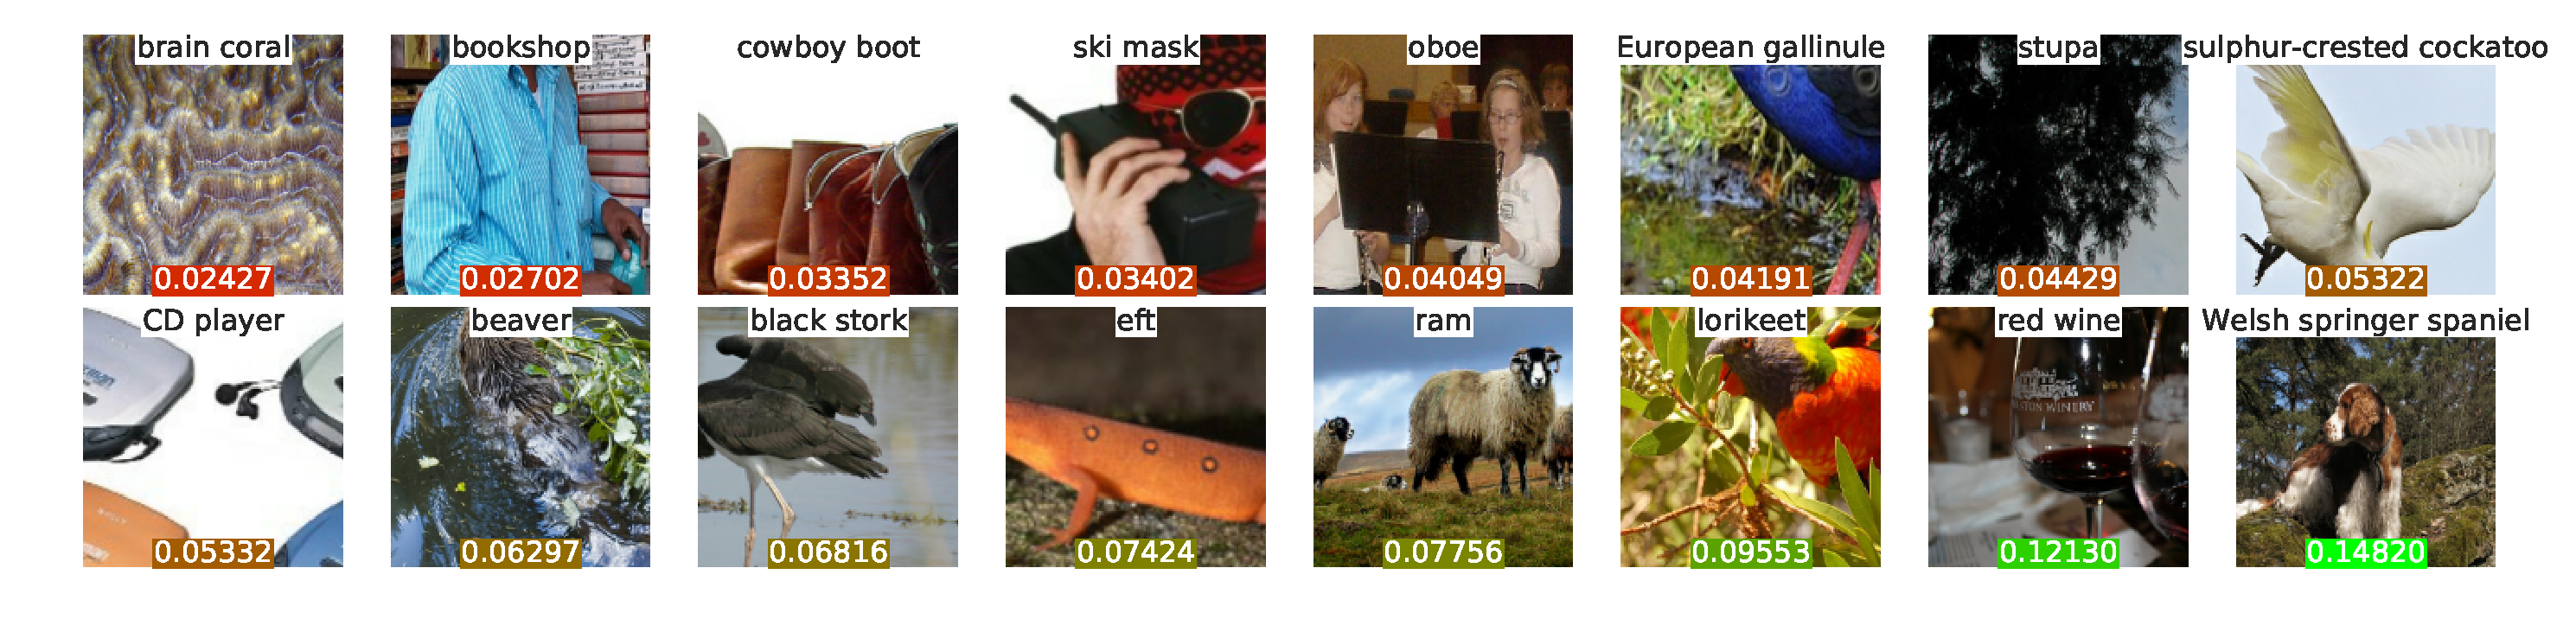
\includegraphics[width=\textwidth]{figs/imagenet_dds.eps}
    %  \vspace{-8mm}
  \caption{\label{fig:dds_score} Example images from the ImageNet and their weights assigned by \dds. A trained DDS scorer assigns higher probabilities to images from ImageNet, in which the class content is more clear. Each image's label and weight in the minibatch is shown.}
   % \vspace{-6mm}
\end{figure*}

\begin{figure}
%\begin{wrapfigure}{r}{0.3\textwidth}
  %\vspace{-12mm}
  %\begin{center}
  \centering
    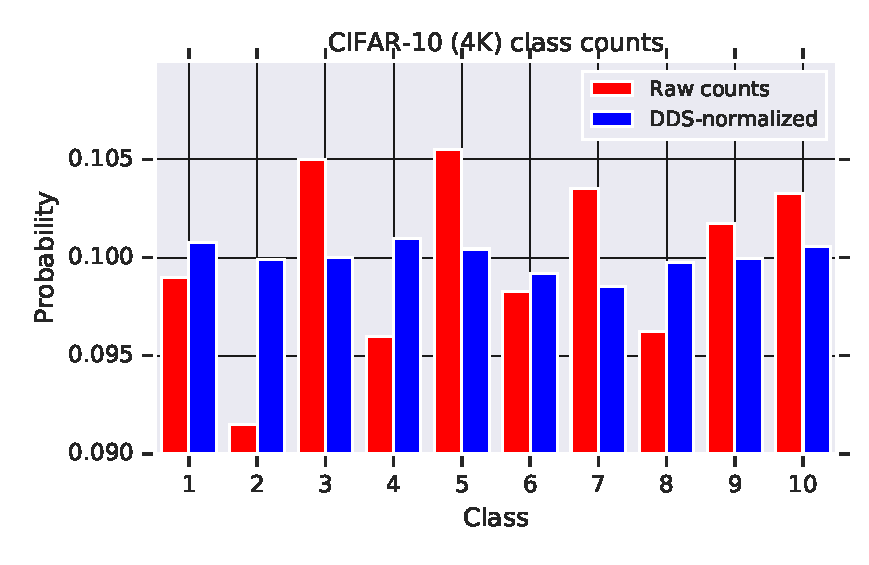
\includegraphics[width=0.4\textwidth]{figs/cifar10_dds.eps}
  %\end{center}
  %\vspace{-4mm}
  %\captionof{figure}{\label{fig:dds_distribution}Class distributions of CIFAR-10 4K.}
  \caption{\label{fig:dds_distribution}A trained DDS scorer learns to balance the class distributions of CIFAR-10 4K.}
  %\vspace{-4mm}
%\end{wrapfigure}
\end{figure}

\begin{figure}
    \centering
    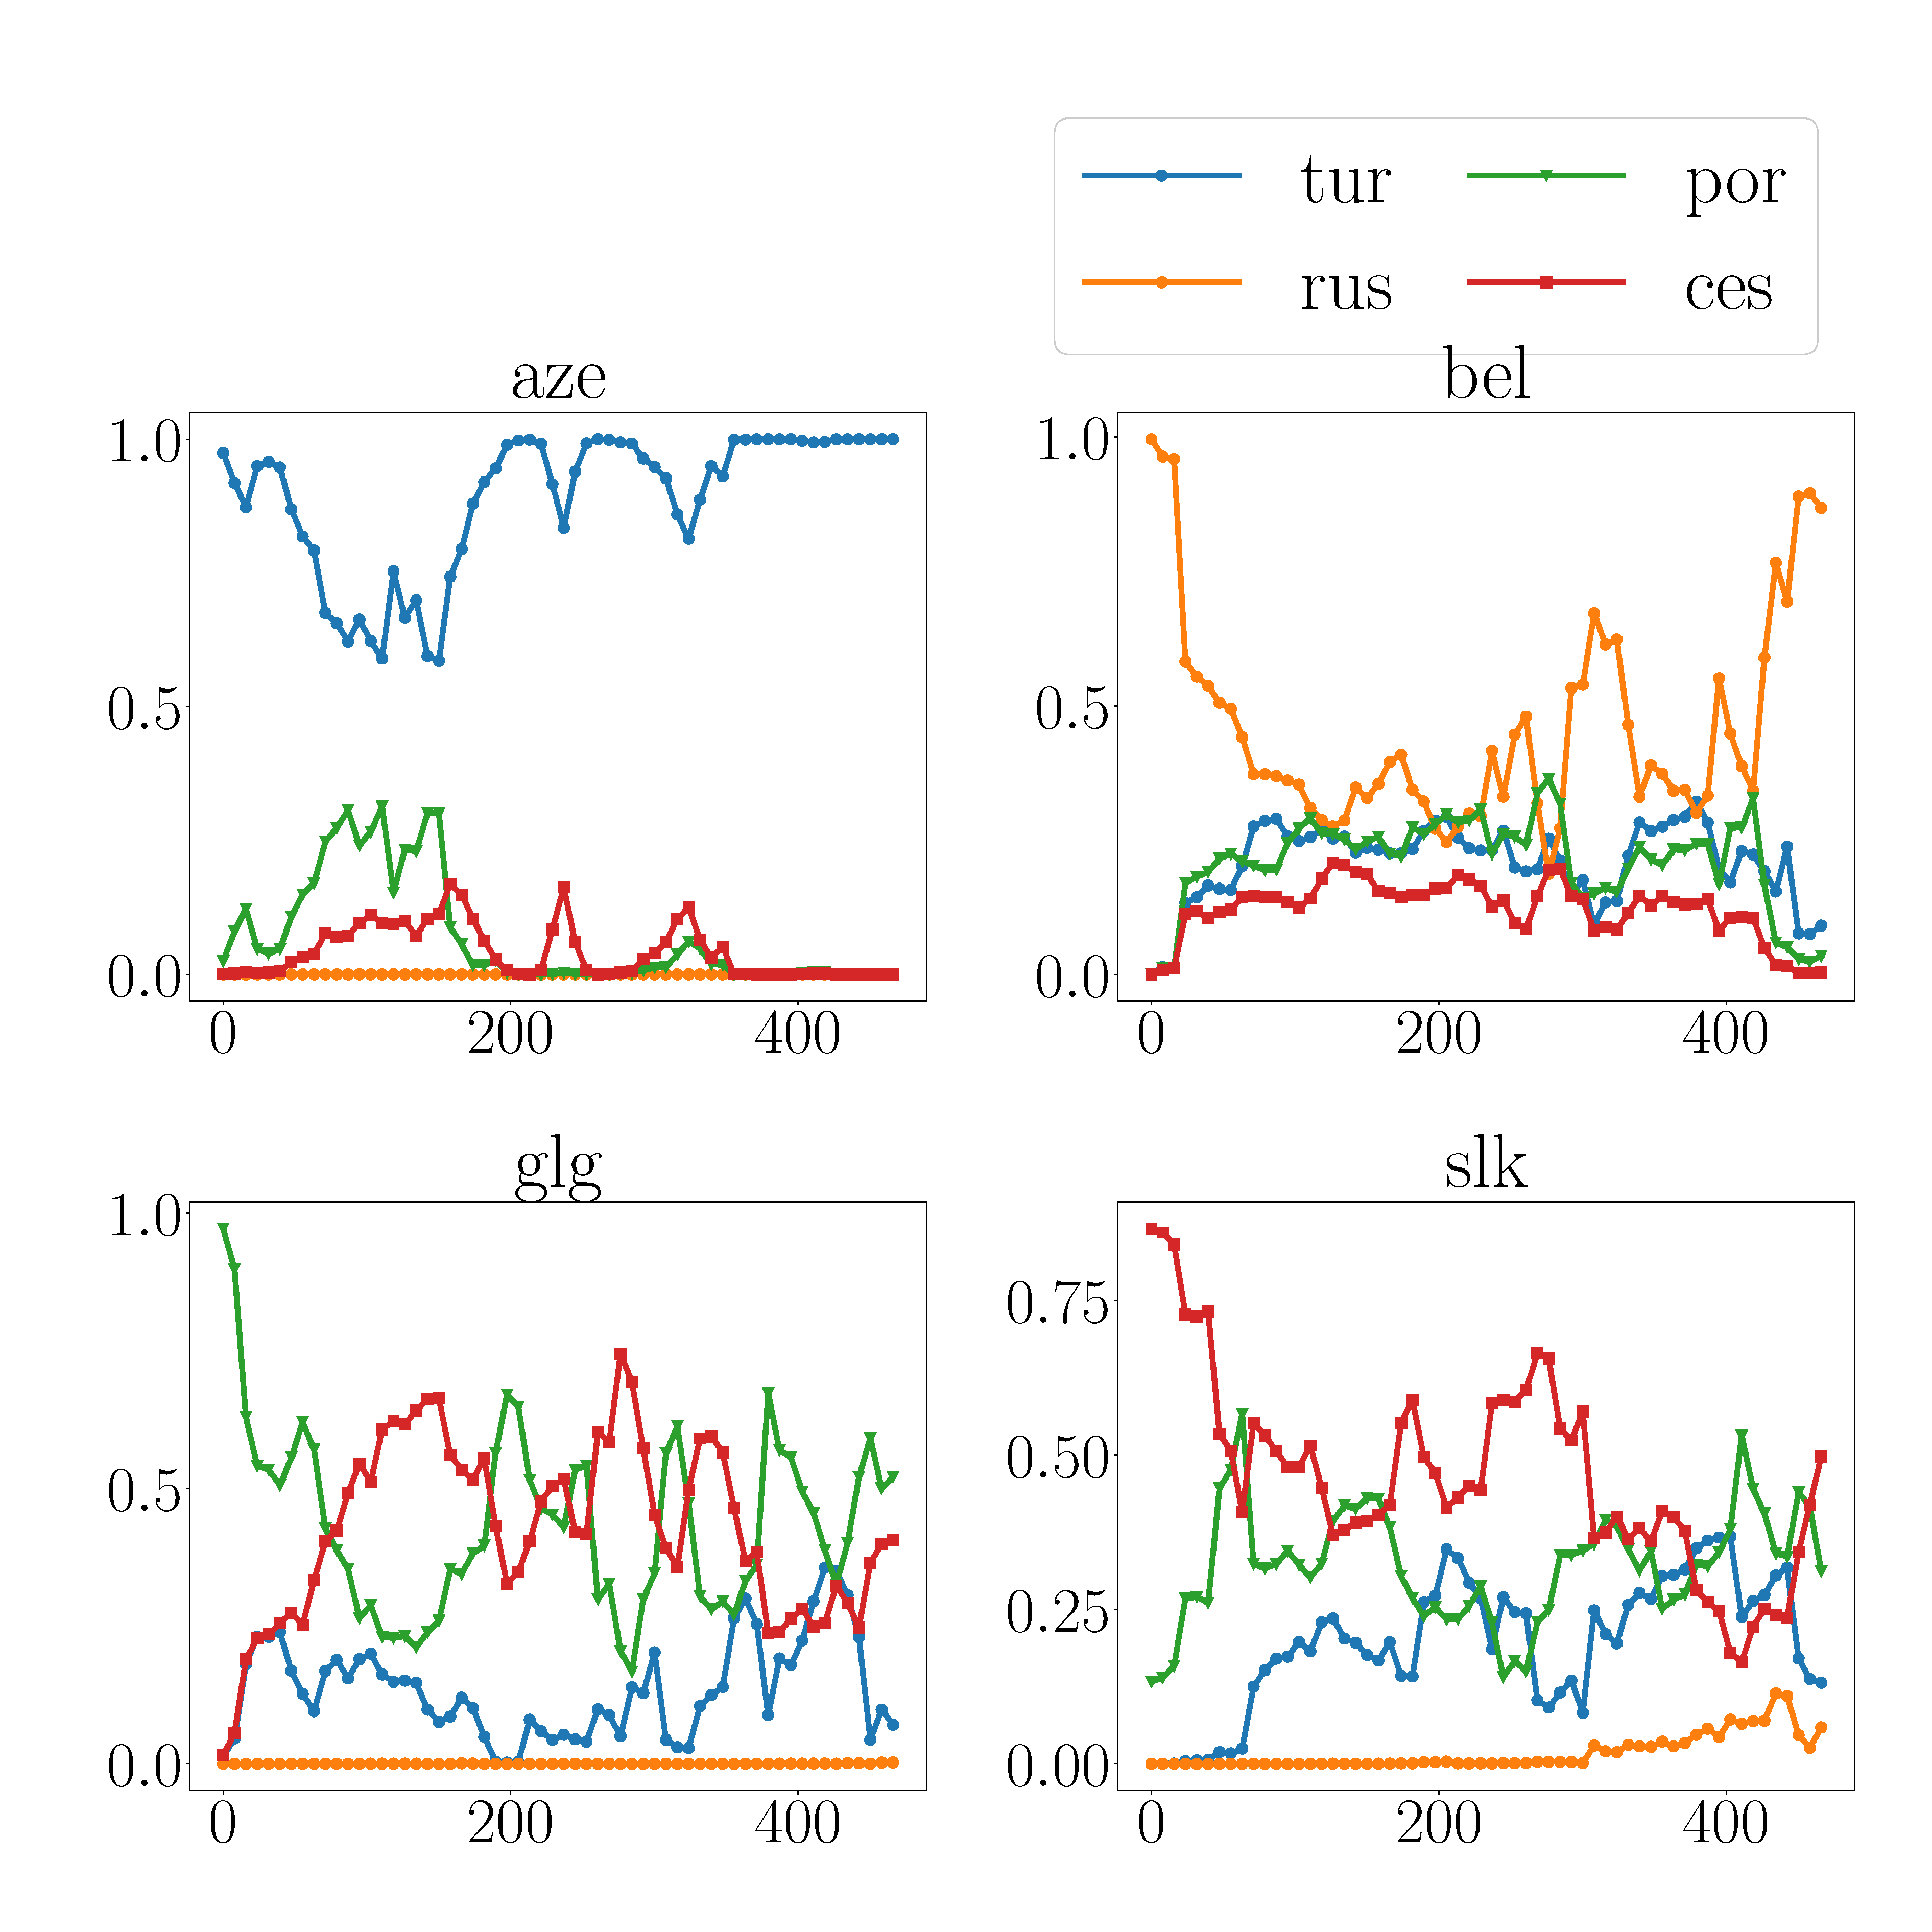
\includegraphics[width=0.9\columnwidth]{figs/hs_prob_plot.eps}
    \caption{\label{fig:nmt_distrib_hs}Language usage for TCS$+$\dds{} by training step. The distribution is initialized to focus on the most related HRL, and \dds~learns to have a more balanced usage of all languages.}
\end{figure}

\subsection{Analysis}


\textbf{Image Classification.} Prior work on heuristic data selection has found that models perform better when fed higher quality or more domain-relevant data  towards the end of training~\citep{dynamic_data_selection_nmt,dynamic}. Here we verify this observation by analyzing the learned importance weight at the end of training for image classification. \autoref{fig:dds_distribution} shows that at the end of training, \dds~learns to balance the class distribution, which is originally unbalanced due to the dataset creation. \autoref{fig:dds_score} shows that at the end of training, \dds~assigns higher probabilities to images with clearer class content from ImageNet. These results show that \dds~learns to focus on higher quality data towards the end of training.  


\textbf{NMT.}
Next, we focus on multilingual NMT, where the choice of data directly corresponds to picking a language, which has an intuitive interpretation. Since \dds~adapts the data weights dynamically to the model throughout training, here we analyze how the dynamics of learned weights.

%\begin{center}
%  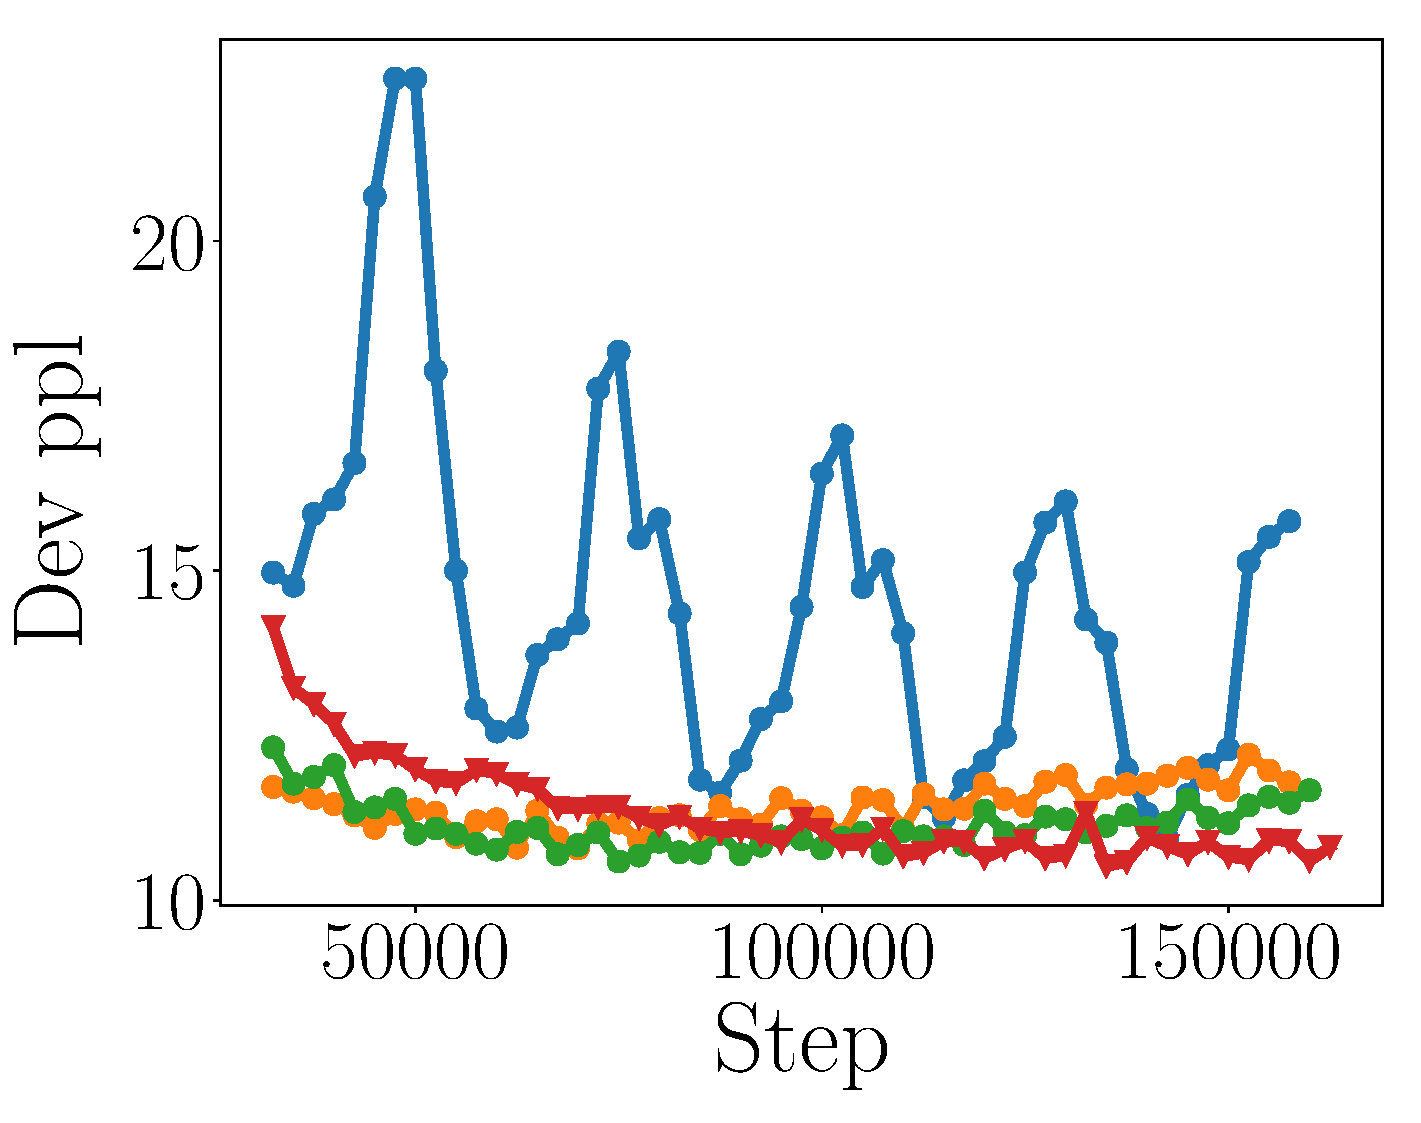
\includegraphics[width=0.245\columnwidth]{figs/aze_devppl_plot.eps}
%  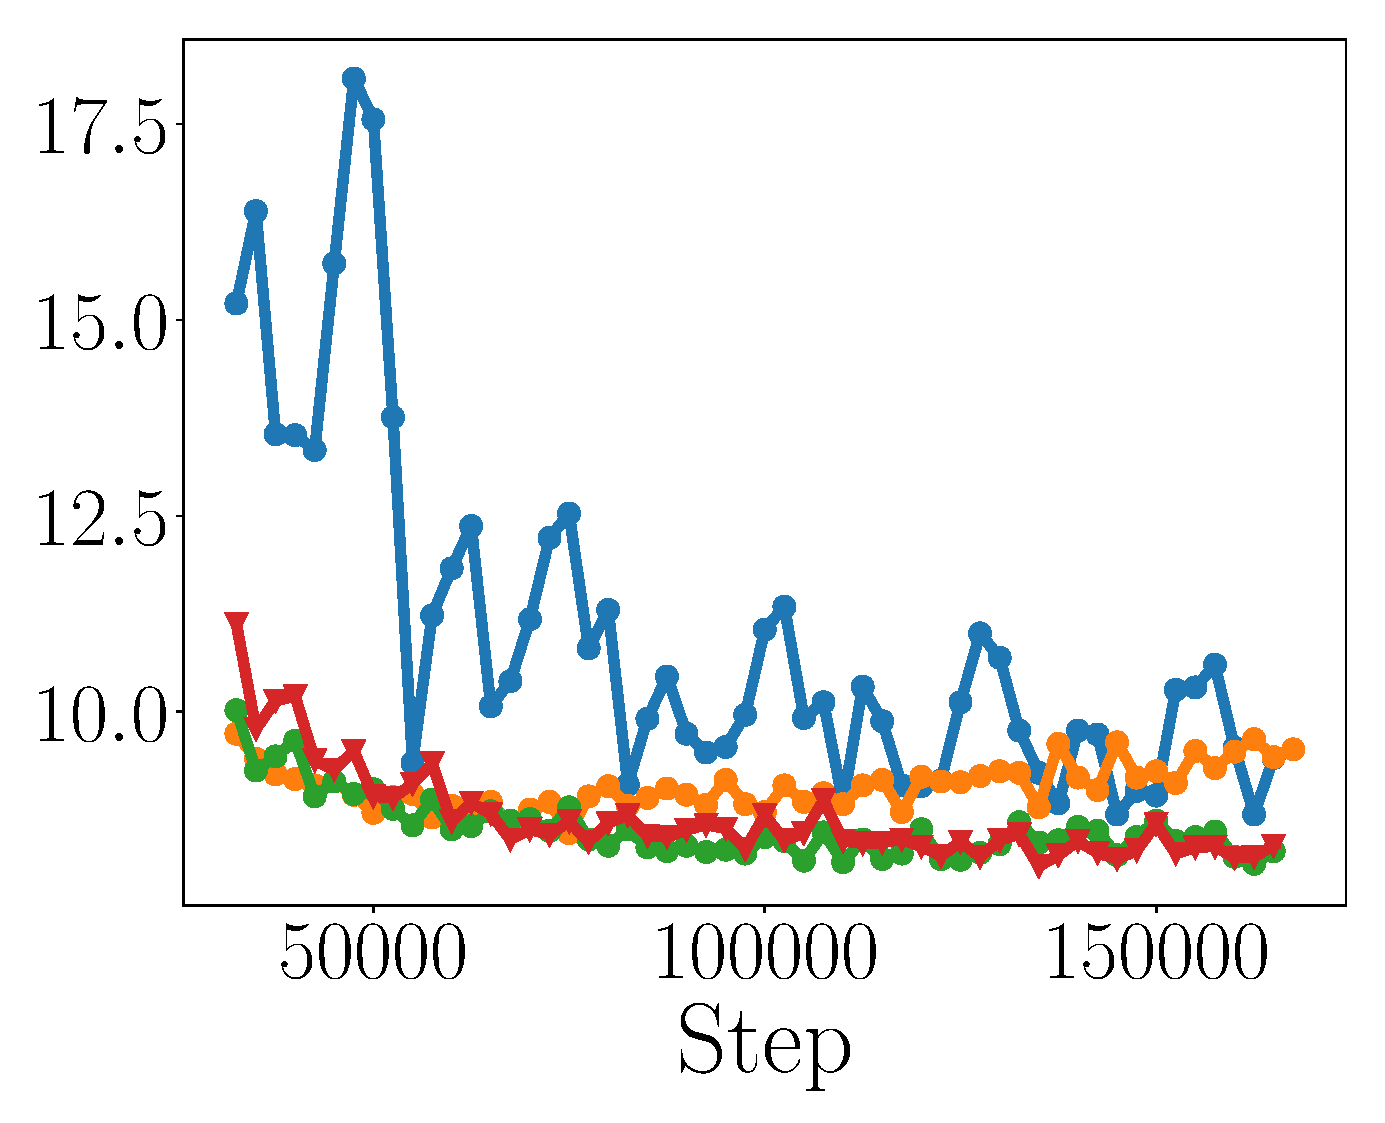
\includegraphics[width=0.23\columnwidth]{figs/bel_devppl_plot.eps}
%  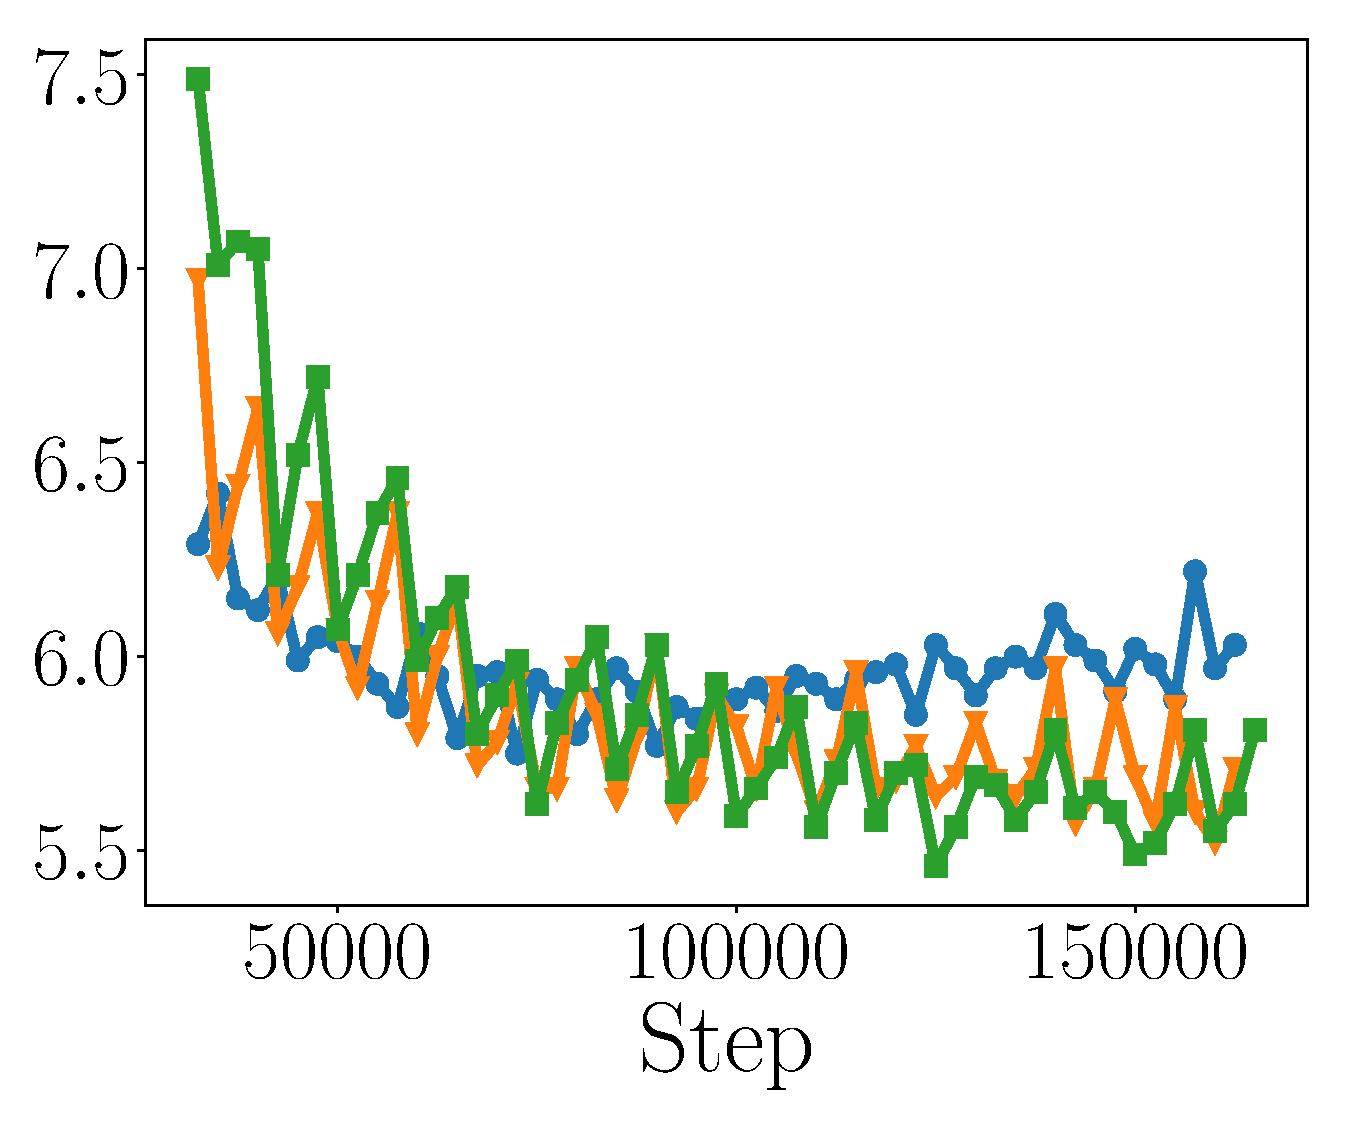
\includegraphics[width=0.23\columnwidth]{figs/glg_devppl_plot.eps}
%  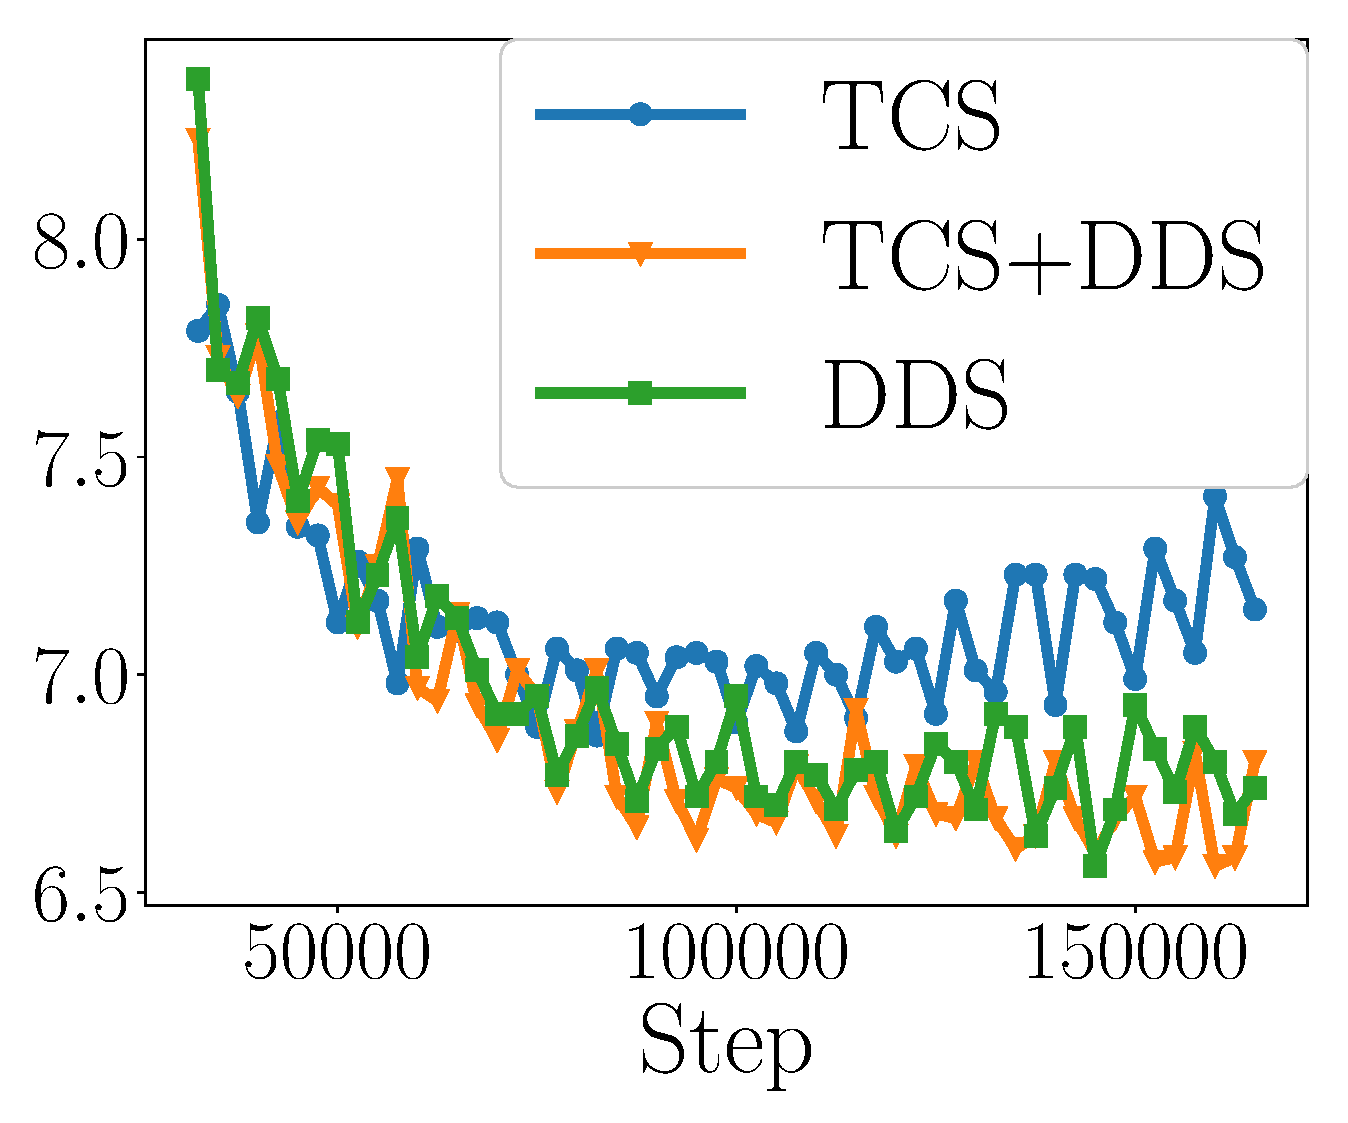
\includegraphics[width=0.23\columnwidth]{figs/slk_devppl_plot.eps}
%  \captionof{figure}{\label{fig:nmt_converge}Development set perplexity vs. training steps. \textit{From left to right}: \texttt{aze}, \texttt{bel}, \texttt{glg}, \texttt{slk}.}
%\end{center}
%\noindent \textbf{Training Curves.} First, we plot the dev set perplexity for three training methods, TCS, DDS, and TCS+DDS over the course of training in Figure \autoref{fig:nmt_converge}.%
%\footnote{We did not plot ``Uniform'' here because it takes a far larger number of training steps to converge due to its uniform sampling of eight different languages, and thus is not visible on the same scale.}
%From the results, we can see that while DDS starts out with a higher perplexity than the TCS heuristics (which a-priori calculates the most appropriate language to be using based on surface statistics), it quickly catches up and surpasses TCS on all 4 languages.
%In addition, when initialized with the TCS heuristic, DDS starts at a relatively good perplexity and converges even faster.

%\begin{center}
%\centering
%  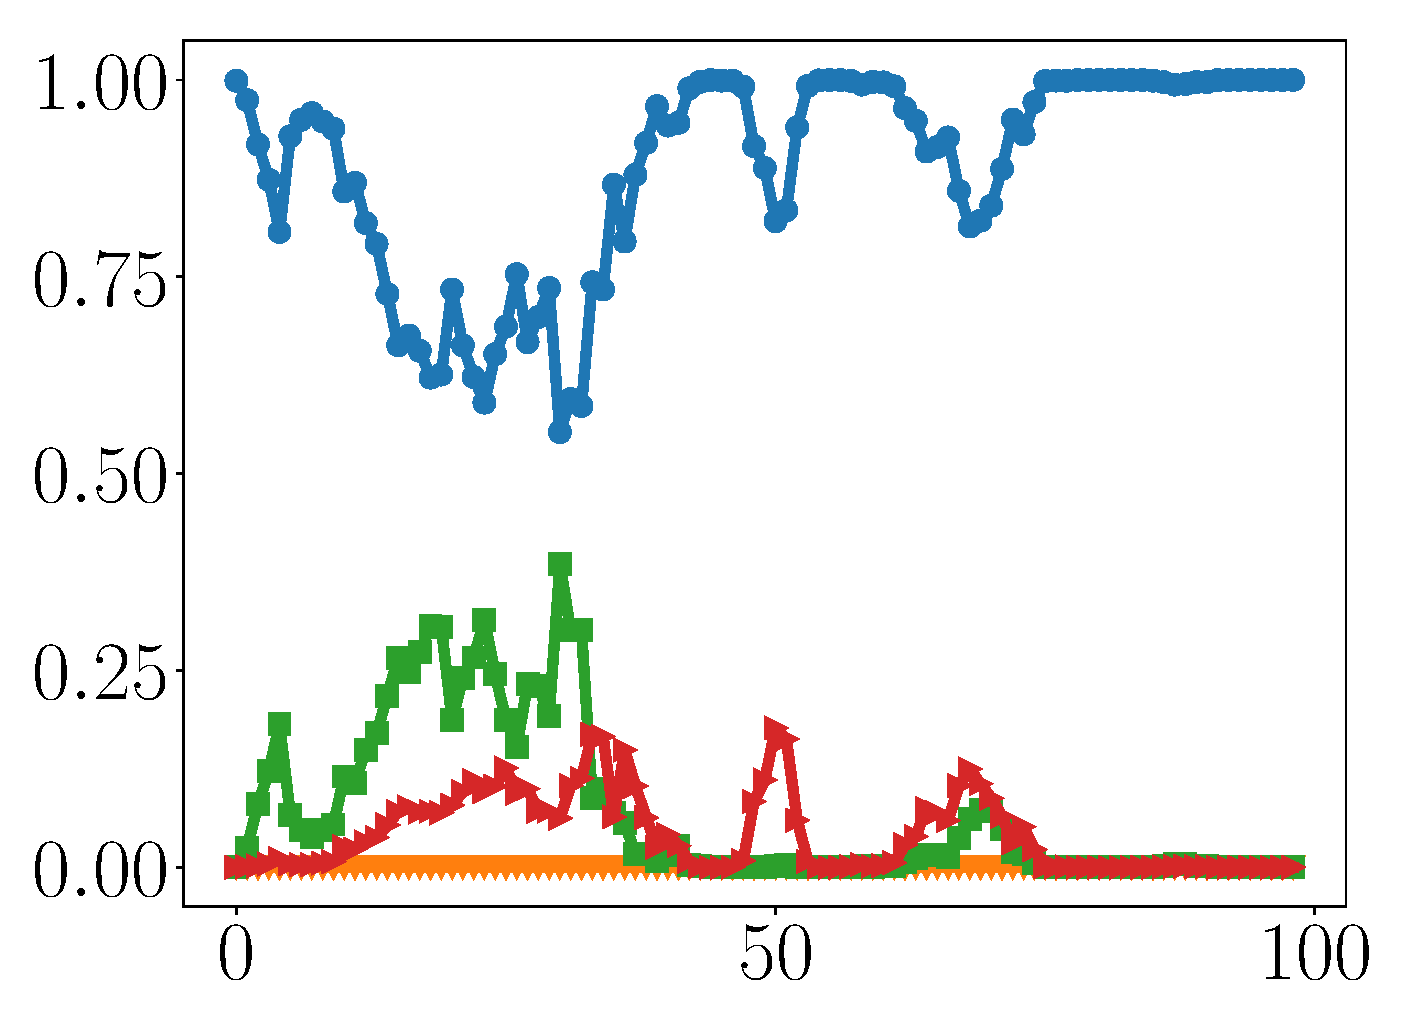
\includegraphics[width=0.4\columnwidth]{figs/aze_hs_probs_plot.eps}
%  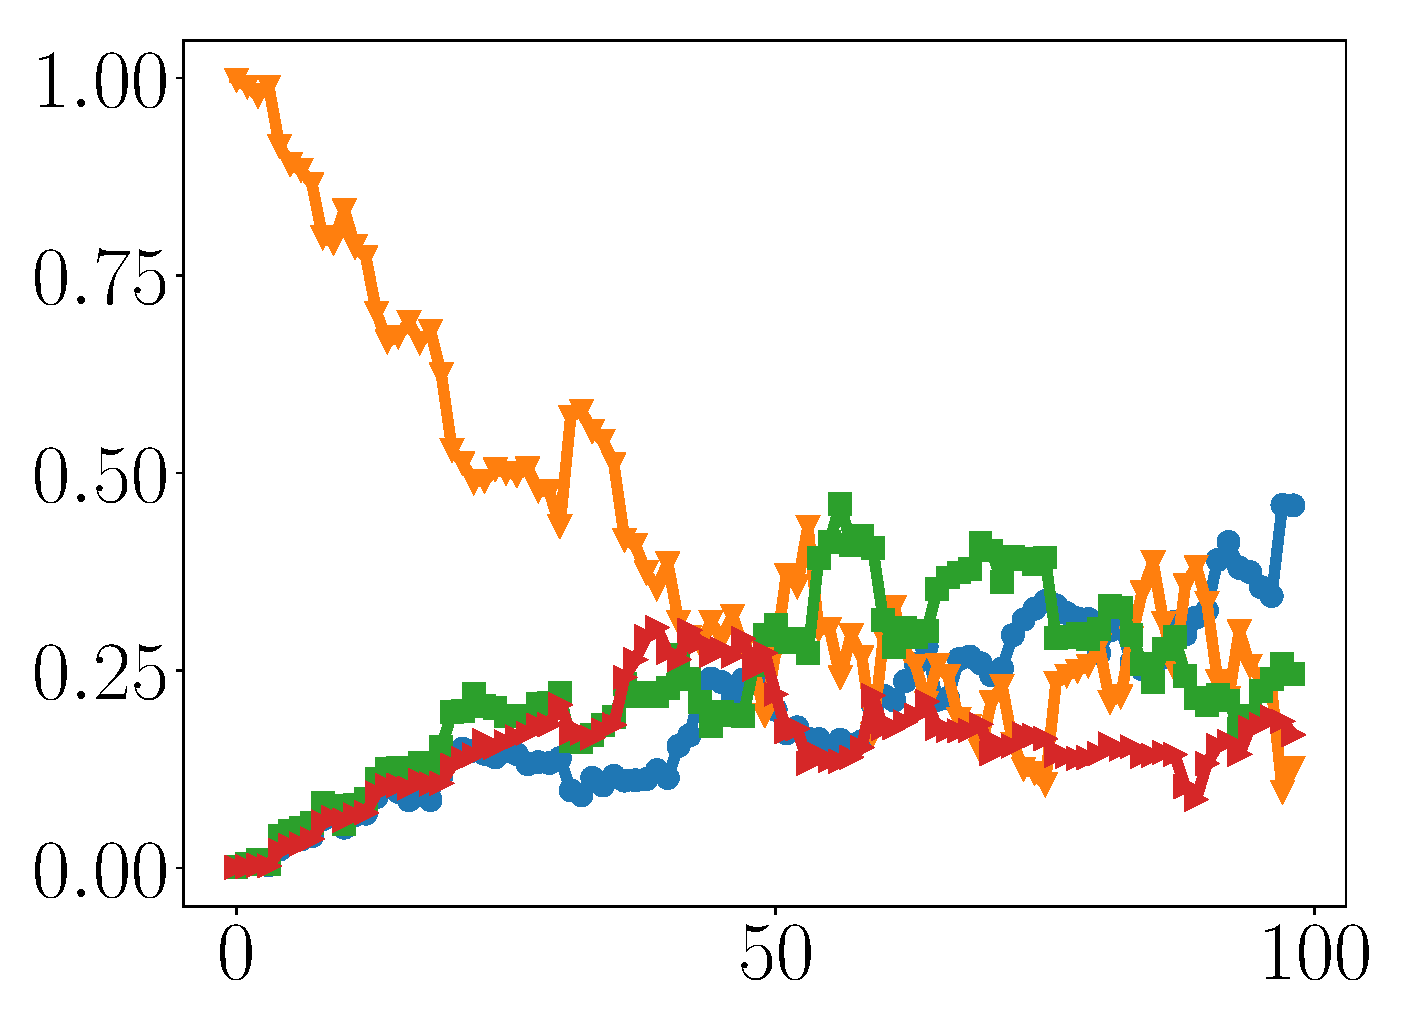
\includegraphics[width=0.4\columnwidth]{figs/bel_hs_probs_plot.eps} \quad\quad\quad\quad
%  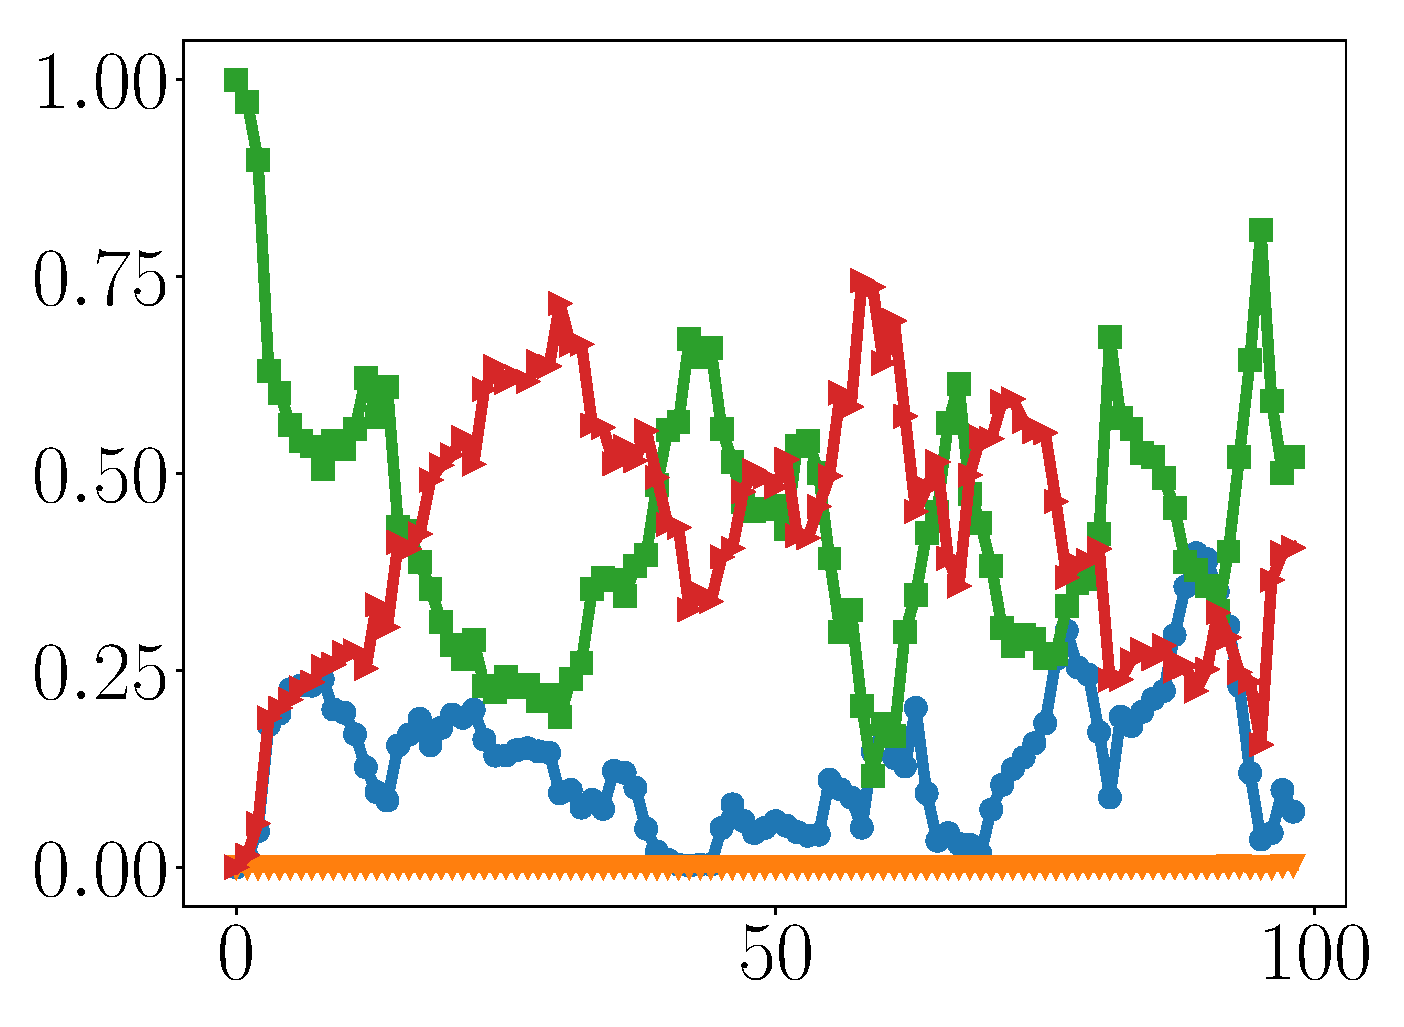
\includegraphics[width=0.4\columnwidth]{figs/glg_hs_probs_plot.eps}
%  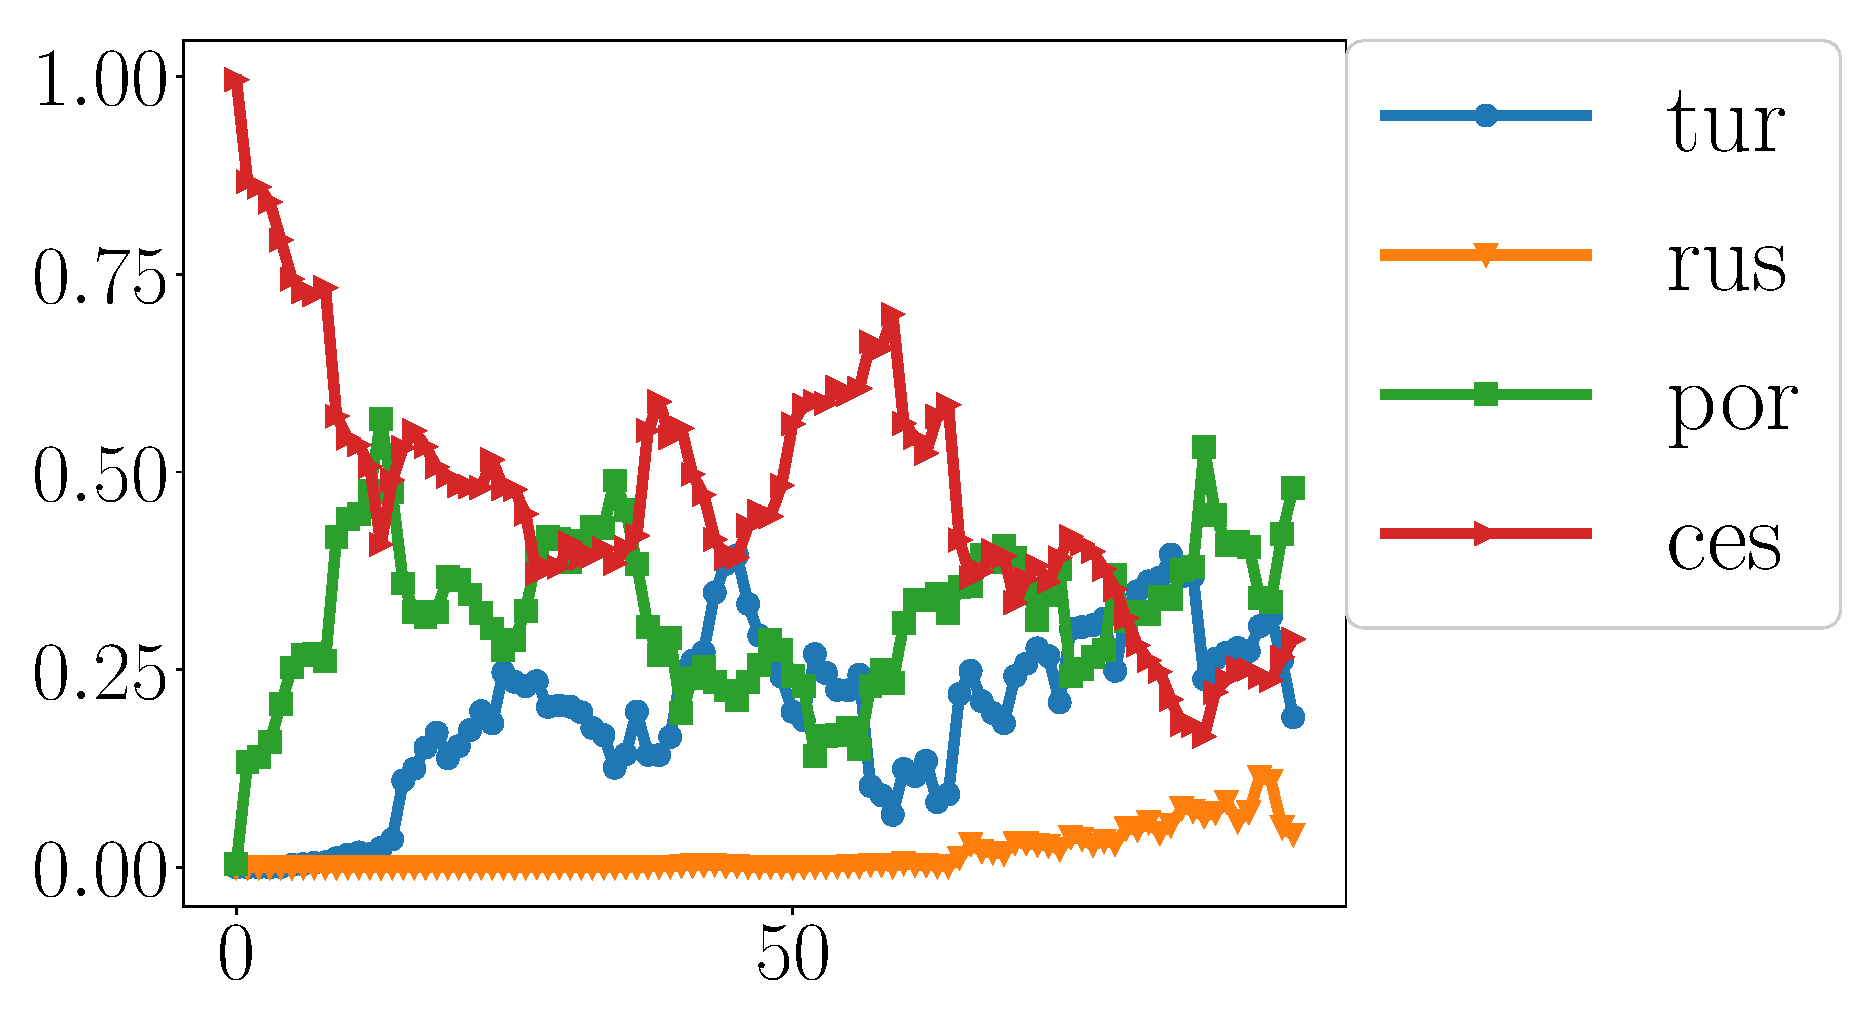
\includegraphics[width=0.5\columnwidth]{figs/slk_hs_probs_plot.eps}
%  %\captionof{figure}{\label{fig:nmt_distrib_hs}Language usage for TCS$+$\dds{} by training step. \textit{From left to right}: \texttt{aze}, \texttt{bel}, \texttt{glg}, \texttt{slk}.}
%  \caption{\label{fig:nmt_distrib_hs}Language usage for TCS$+$\dds{} by training step. \textit{From left to right}: \texttt{aze}, \texttt{bel}, \texttt{glg}, \texttt{slk}.}
%\end{center}
\begin{figure}
    \centering
    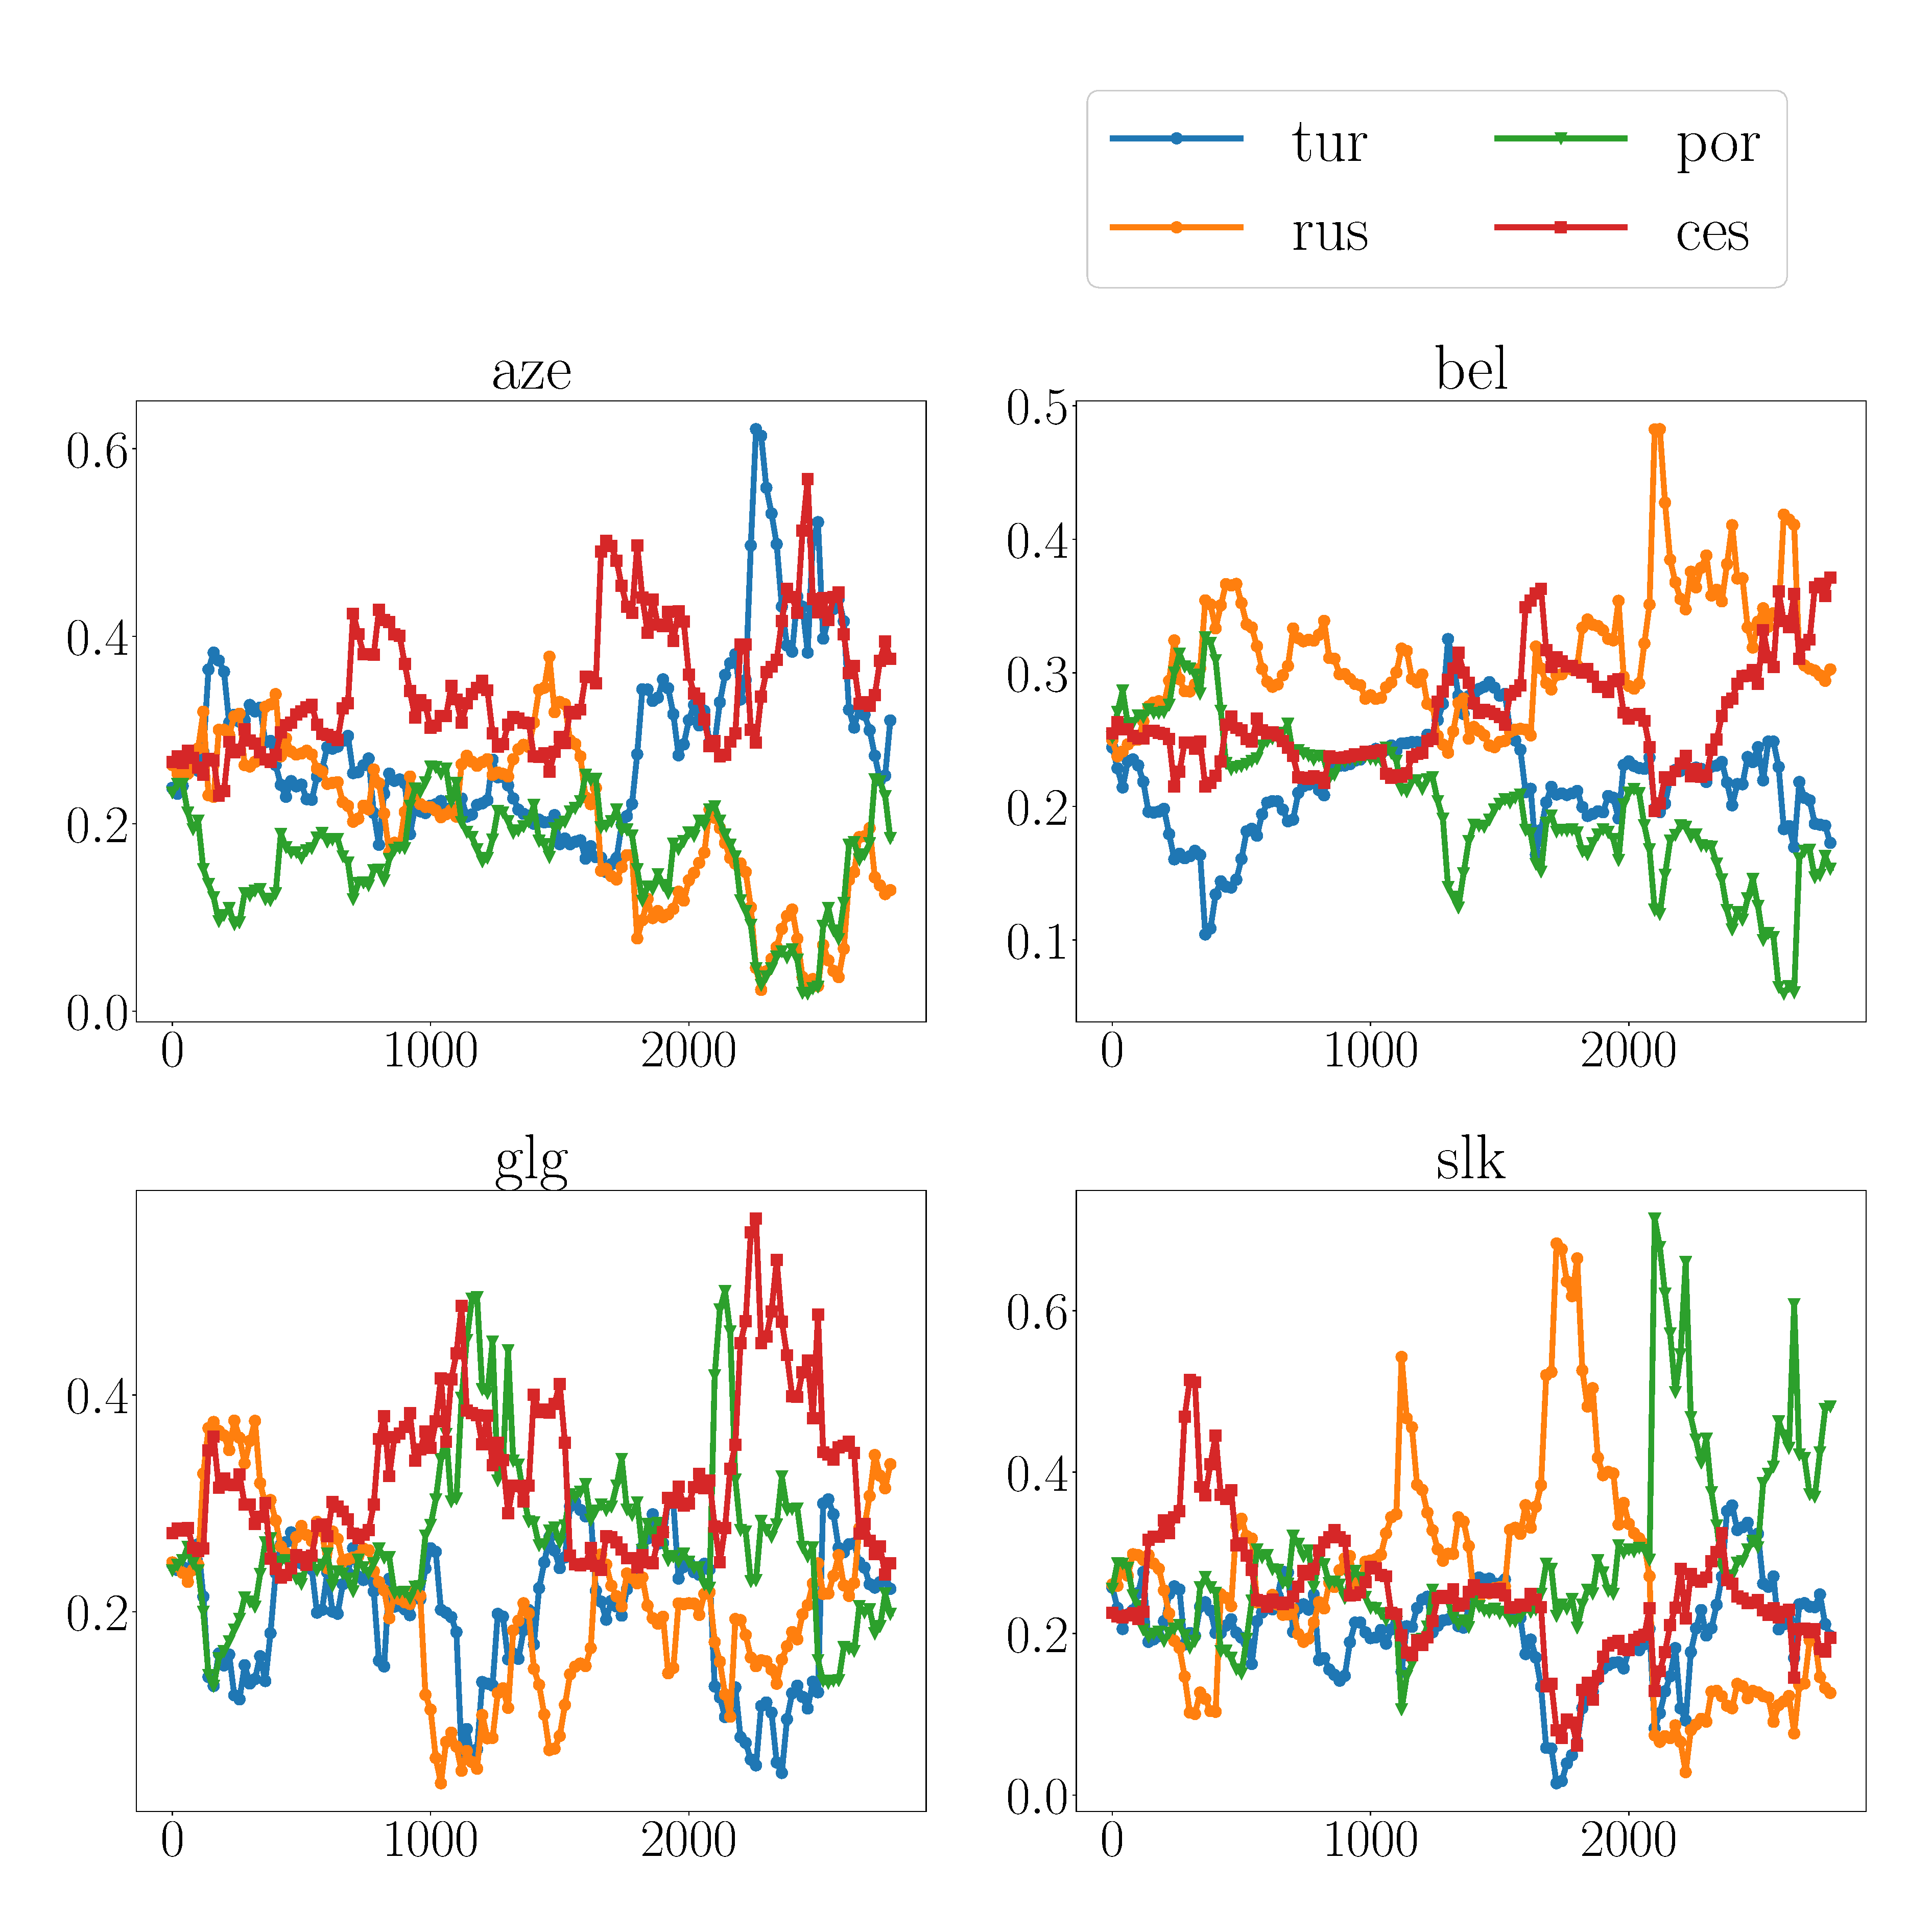
\includegraphics[width=0.9\columnwidth]{figs/uniform_prob_plot.eps}
    \caption{\label{fig:nmt_distrib_uni}Language usage for \dds~by training step. \dds~learns to upweight the most related HRL after certain training steps.}
    \vspace{-6mm}
\end{figure}
%\noindent \textbf{Learned Language Distributions.}
We plot the probability distribution of the four HRLs (because they have more data and thus larger impact on training) over the course of training.  \autoref{fig:nmt_distrib_hs} shows the change of language distribution for TCS+DDS. Since TCS selects the language with the largest vocabulary overlap with the LRL, the distribution is initialized to focus on the most related HRL. For all four LRLs, the percentage of their most related HRL starts to decrease as training continues. For \texttt{aze}, \dds~quickly comes back to using its most related HRL. For \texttt{gig} and \texttt{slk}, DDS learns to mainly use both \texttt{por} and \texttt{ces}, their corresponding HRL. However, for \texttt{bel}, \dds~continues the trend of using all four languages. This shows that \dds~is able to maximize the benefits of the multilingual data by having a more balanced usage of all languages. 


%For gig and slk, DDS learns to mainly use both por and ces, their corresponding HRL.

\autoref{fig:nmt_distrib_uni} shows a more interesting trend of \dds~without heuristic initialization.
For both \texttt{aze} and \texttt{bel}, \dds~focuses on the most related HRL after a certain number of training updates.
Interestingly, for \texttt{bel}, \dds~learns to focus on both \texttt{rus}, its most related HRL, and \texttt{ces}. Similarly for \texttt{slk}, \dds~also learns to focus on \texttt{ces}, its most related HRL, and \texttt{rus}, although there is little vocabulary overlap between \texttt{slk} and \texttt{rus}.
Also notably, the ratios change  significantly over the course of training, indicating that different types of data may be more useful during different learning stages.


%\vspace{-0.2cm}
%\begin{center}
%  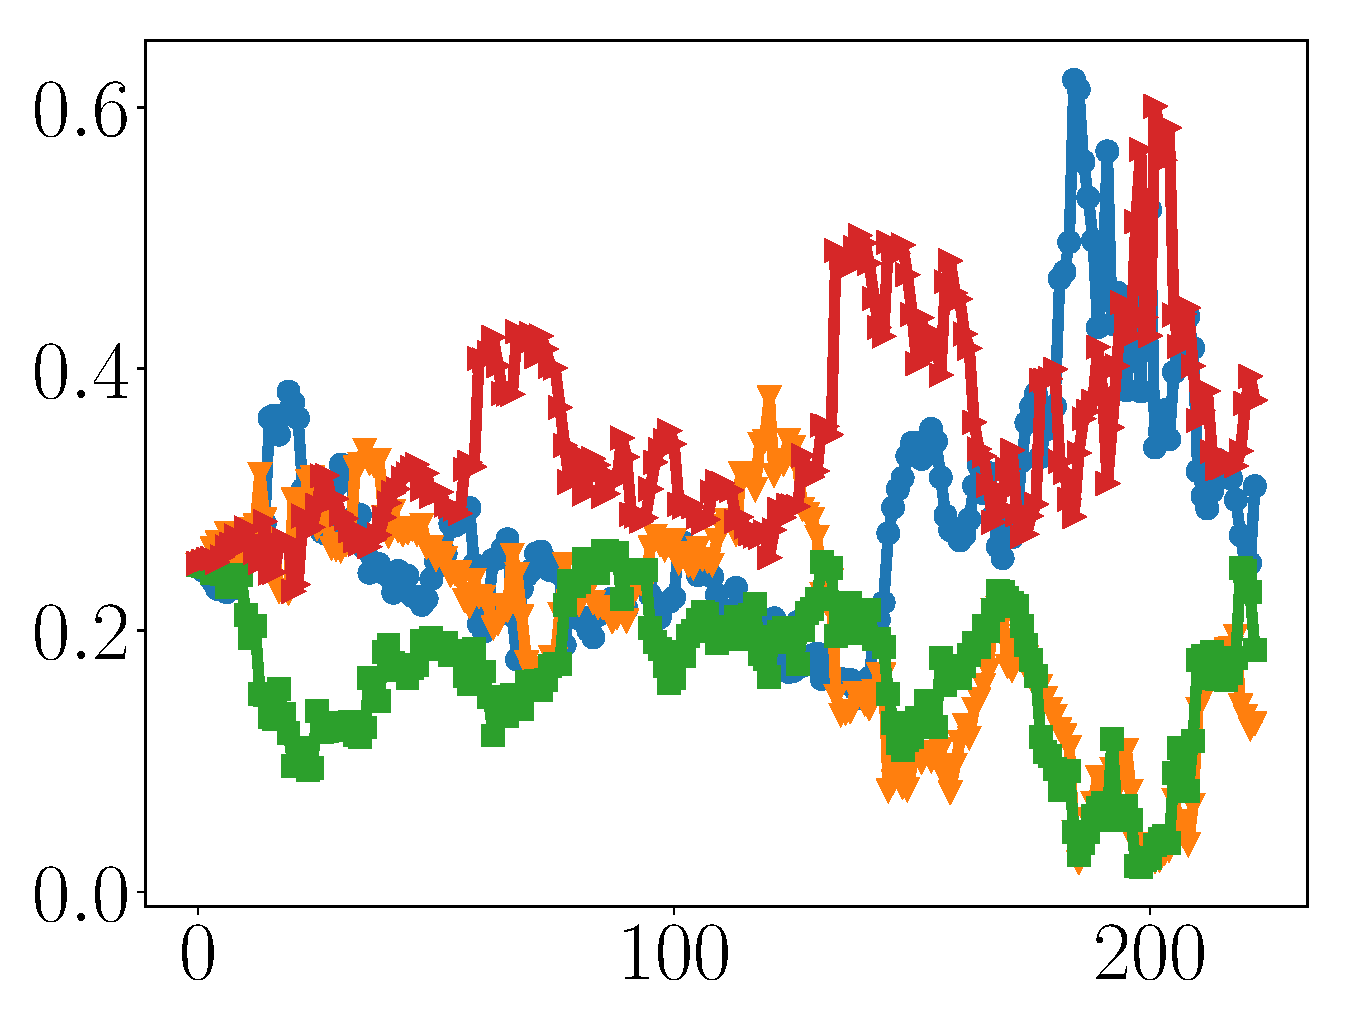
\includegraphics[width=0.20\columnwidth]{figs/aze_uni_probs_plot.eps}
%  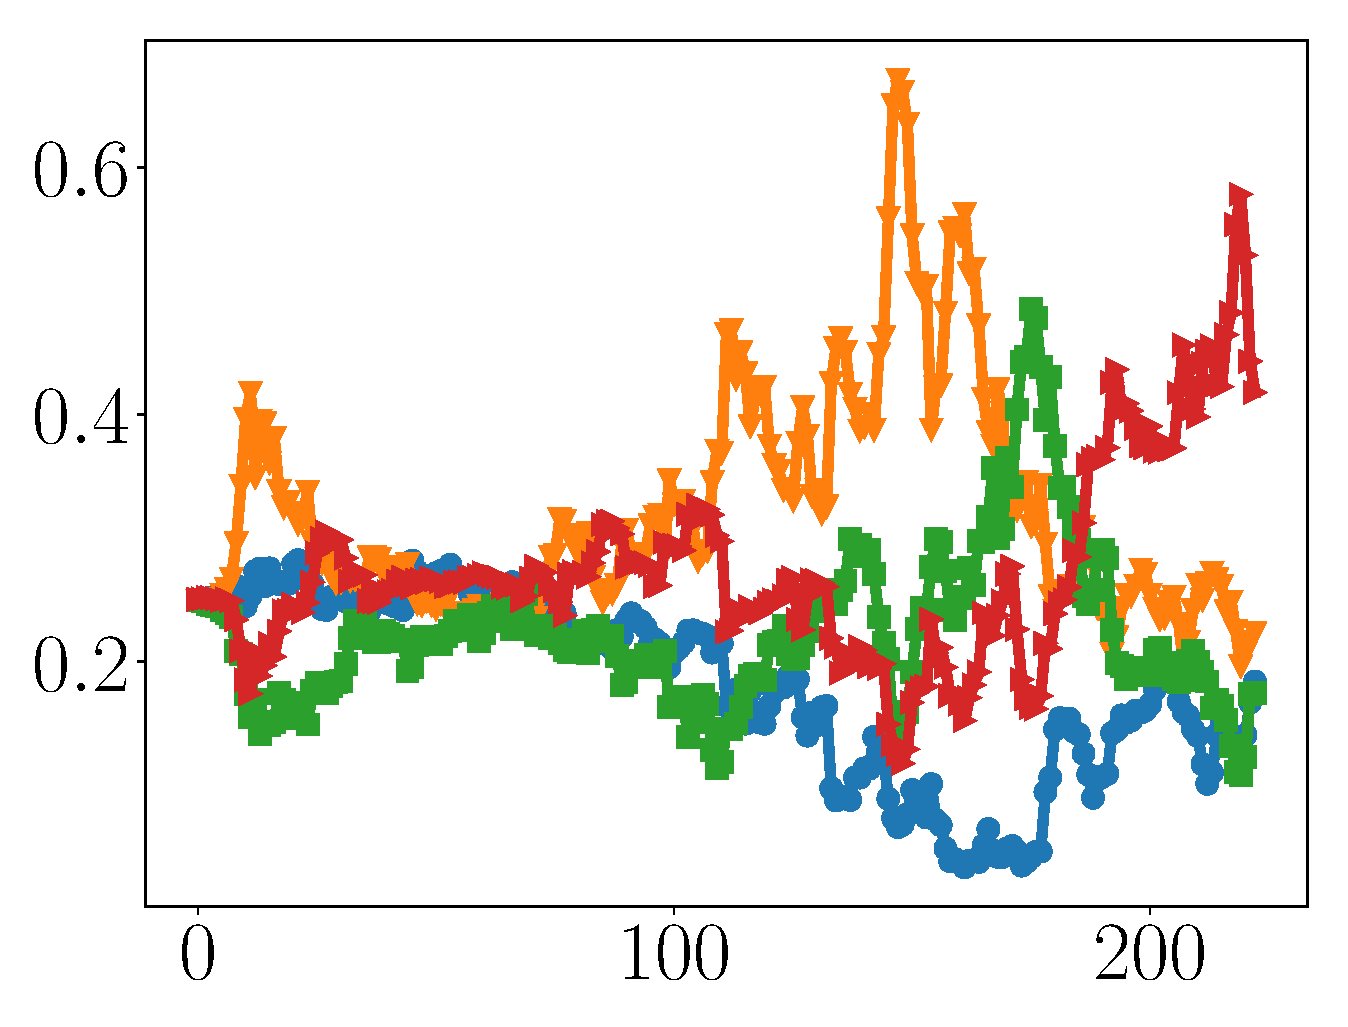
\includegraphics[width=0.20\columnwidth]{figs/bel_uni_probs_plot.eps}
%  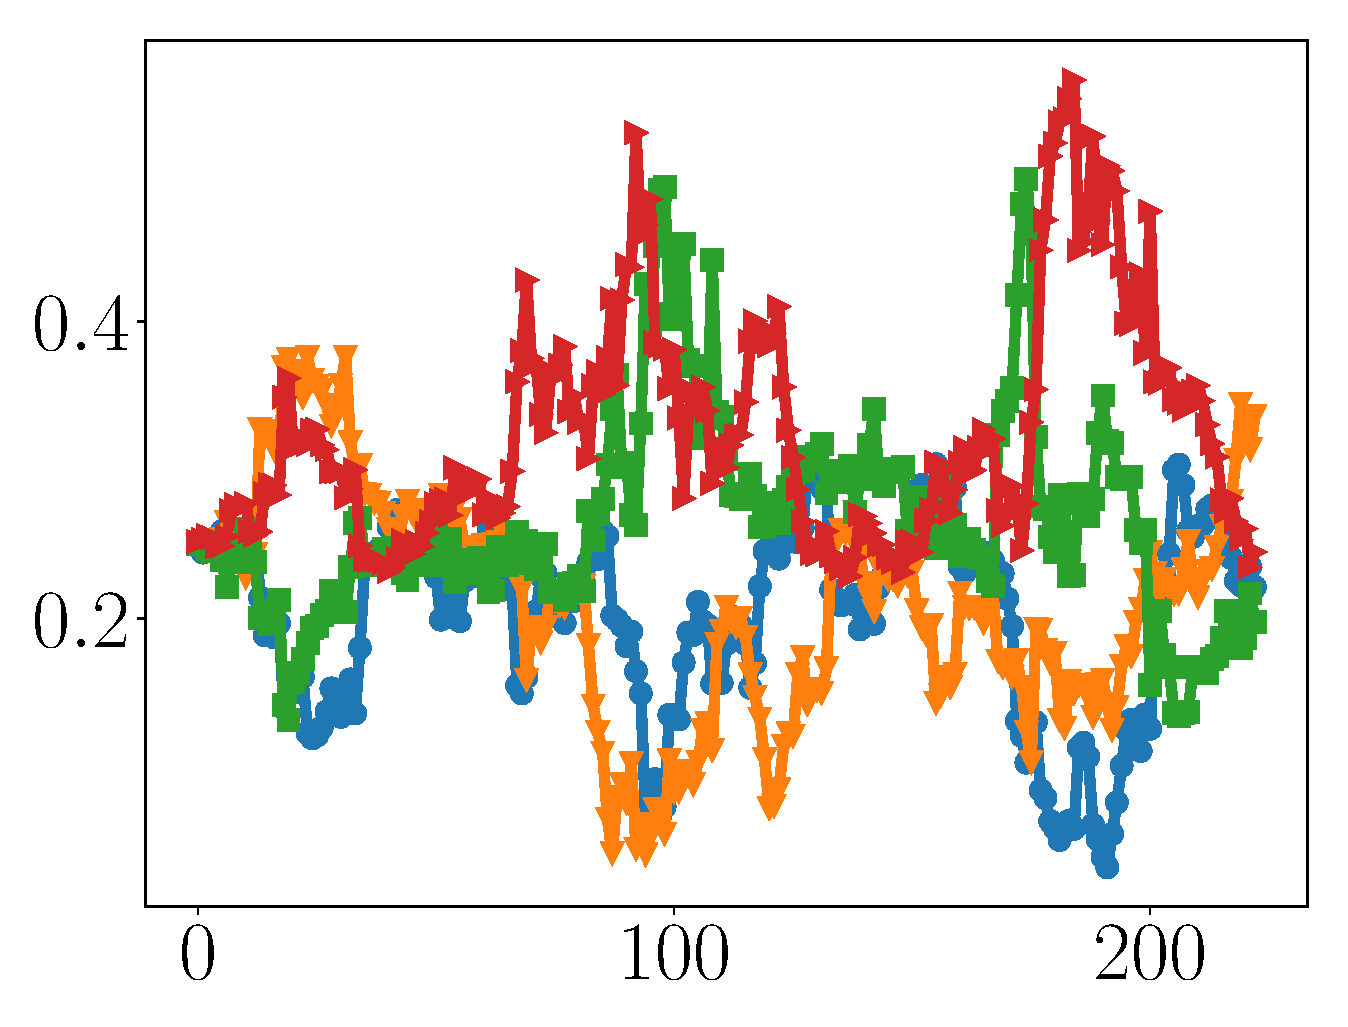
\includegraphics[width=0.2\columnwidth]{figs/glg_uni_probs_plot.eps}
%  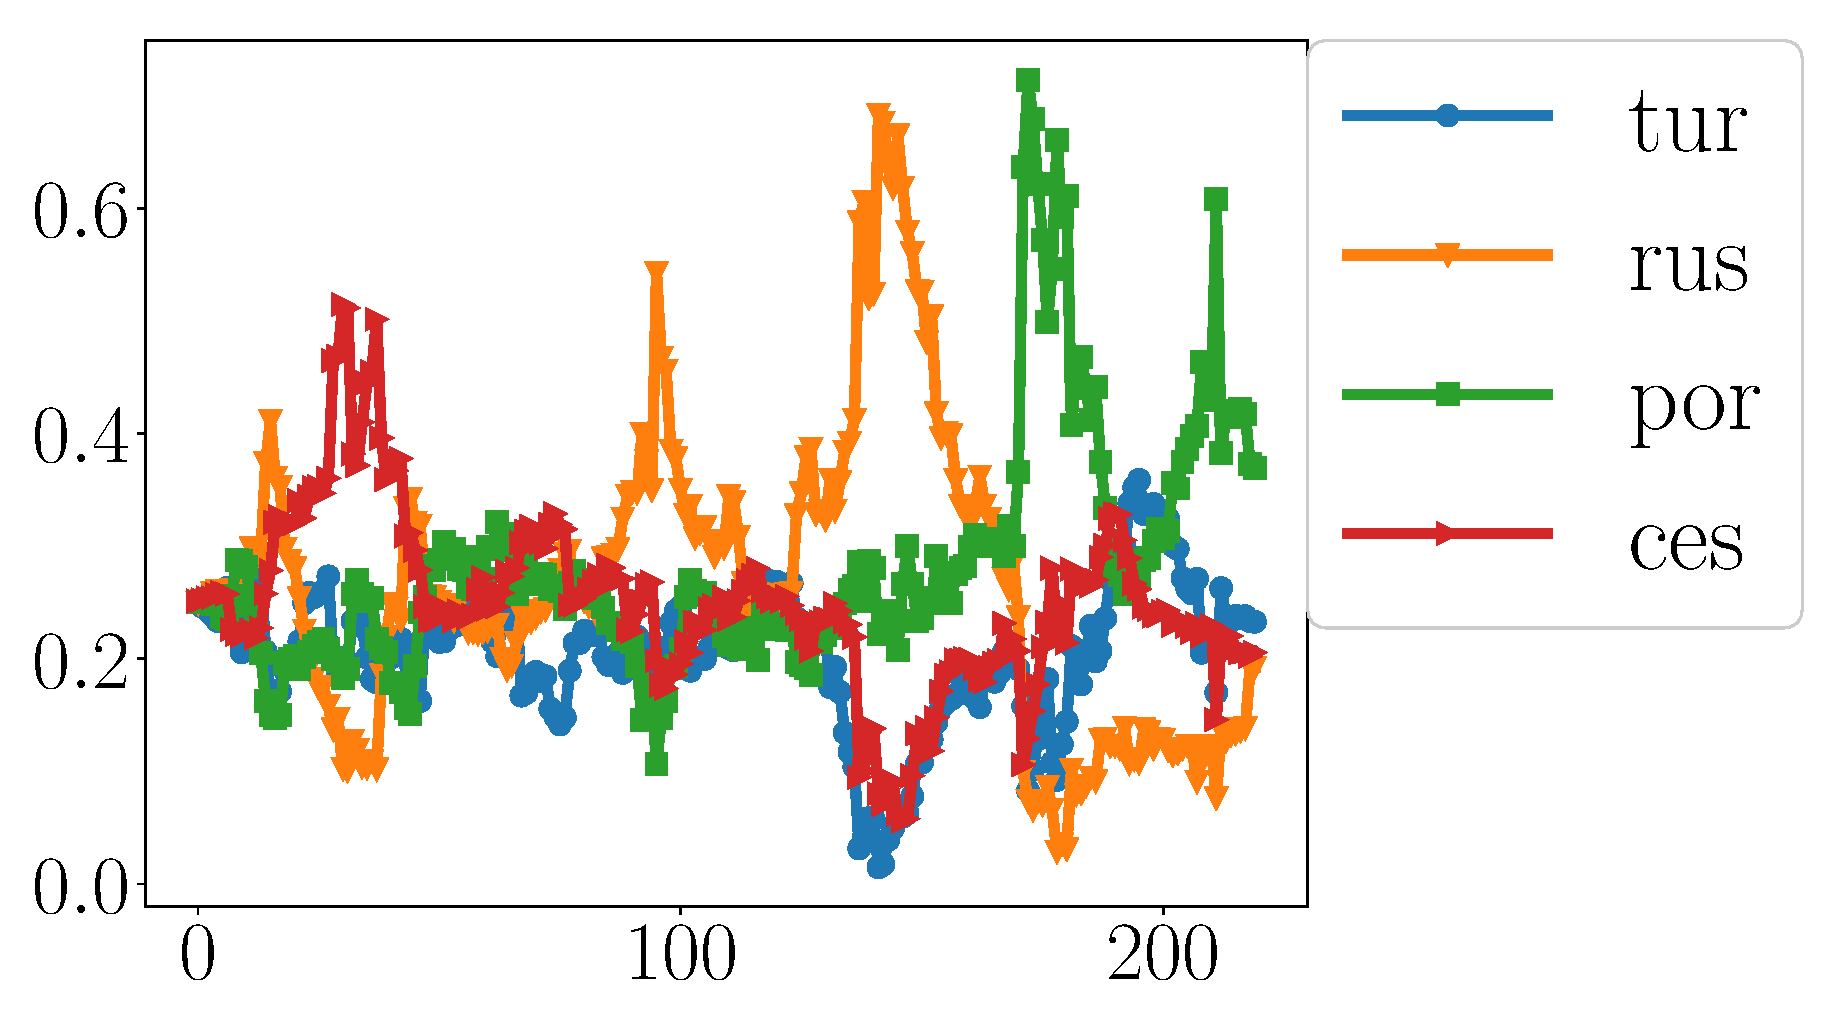
\includegraphics[width=0.25\columnwidth]{figs/slk_uni_probs_plot.eps}
%  \vspace{-0.1cm}
%  \captionof{figure}{\label{fig:nmt_distrib_uni}Language usage for \dds~by training step. \textit{From left to right}: \texttt{aze}, \texttt{bel}, \texttt{glg}, \texttt{slk}.}
%\end{center}
%\vspace{-0.1cm}


% This indicate that \dds~is able to discover the best data to use even if the patterns are not immediately intuitive.
%Similar to the trend in Figure \autoref{fig:nmt_distrib_hs}, glg tends to use both por, its most related HRL, and ces. 

\section{\label{sec:related_work}Related Work}
\paragraph{Data Selection Methods} Data selection for domain adaptation for disparate tasks has also been extensively studied~\citep{moore2010intelligent,axelrod2011domain,domain_adapt_transfer,jiang-zhai-2007-instance,foster-etal-2010-discriminative,wang-etal-2017-instance}. These methods generally design heuristics to measure domain similarity.
\cite{domain_adapt_transfer} propose to estimate the importance weight of the classification labels in the pretraining dataset to mitigate the domain differences, while \dds~is a more general data selection framework that works for both classification and other usage cases. Besides domain adaptation, selecting also benefits training in the face of noisy or otherwise undesirable data~\citep{vyas-etal-2018-identifying,pham-etal-2018-fixing}. 

Submodular optimization~\citep{submodular_mt,learn_mix_submodular} selects training data that are similar to dev set, but the criterion is often based on hand-designed features and the data usage is predefined before training. However, \dds~directly optimizes the the dev set performance, and is generalizable across tasks. Moreover, unlike \dds, these methods cannot adaptively change the data selection scheme. 
%The idea of selecting training data that are similar to dev data has been used in works on submodular optimization~\citep{submodular_mt,learn_mix_submodular}, but they rely on features specific to the task, while \dds~directly optimizes the the dev set performance, and is generalizable across tasks. Moreover, unlike \dds, these methods cannot adaptively change the data selection scheme. 


\paragraph{Instance Weighting Methods} Our method is also related to works on training instance weighting~\citep{importance_weight,learn_reweight,jiang-zhai-2007-instance,domain_adapt_transfer}. These methods reweigh data based on a manually computed weight vector, instead of using a parameterized neural network.
Notably,~\citet{learn_reweight} tackles noisy data filtering for image classification, by using meta-learning to calculate a locally optimized weight vector for each batch of data.
In contrast, our work focuses on the general problem of optimizing data usage. We train a parameterized scorer network that optimizes over the entire data space, which can be essential in preventing overfitting mentioned in ~\autoref{sec:method};  empirically our method outperform \cite{learn_reweight} by a large margin in ~\autoref{sec:experiment}. \cite{importance_weight} optimizes data weights by minimizing the error rate on the dev set. However, they use a single number to weigh each subgroup of augmented data, and their algorithm requires an expensive heuristic method to update data weights; while \dds~uses a more expressive parameterized neural network to model the individual data weights, which are efficiently updated by directly differentiating the dev loss.
%\gn{Here we should discuss \cite{learn_reweight} in detail, so that we can explain the difference for people who are familiar with this paper. Specifically (1) our work is parameterized and parameters are amortized over the entire dataset, which may be essential in preventing the overfitting mentioned in Section \autoref{diff_data_selection}, (2) our work is not only focused at filtering noisy data, and (3) it empirically performs better.}
 
 \paragraph{Curriculum Learning} Many machine learning approaches consider how to best present data to models. First, difficulty-based curriculum learning estimates the presentation order based on heuristic understanding of the hardness of examples~\citep{cl_bengio,SpitkovskyAJ10,baysian_curriculum,zhang2016boosting,automate_cl_GravesBMMK17,zhang2018empirical,platanios19naacl}. These methods, though effective, often generalize poorly because they require task-specific difficulty measures. On the other hand, self-paced learning~\citep{spl_kumar,spl_visual_category} defines the hardness of the data based on the loss from the model, but is still based on the assumption that the model should learn from easy examples. Our method does not make these assumptions. 

 \paragraph{RL for Training Data Usage} Our method is closest to the learning to teach framework~\citep{learn_to_teach} but their formulation involves manual feature design and requires expensive multi-pass optimization. Instead, we formulate our reward using bi-level optimization, which has been successfully applied for a variety of other tasks~\citep{bilevel_optim,hier_optim,darts,hyper_grad,learn_reweight}. \citep{reinforce_cotrain,rl_nmt,learn_active_learn} propose RL frameworks for specific natural language processing tasks, but their methods are less generalizable and requires more complicated featurization.





%Instance weighting: \cite{jiang-zhai-2007-instance,foster-etal-2010-discriminative,wang-etal-2017-instance}. In particular, \cite{wang-etal-2017-instance} seems like a good paper to compare against because it's recent and based on neural MT.

%Curriculum learning: \cite{zhang2016boosting,zhang2018empirical,platanios19naacl}.

%Data selection: \cite{moore2010intelligent,axelrod2011domain}.

%Removing bad training examples improves MT: \cite{vyas-etal-2018-identifying,pham-etal-2018-fixing}

%Dataset poisoning (for neural models): \cite{koh2017understanding}



%Meta-learning. Formulation of using the gradient update equation is similar to MAML \cite{finn2017model}.

\section{\label{sec:conclusion}Conclusion}
We present Differentiable Data Selection, an efficient RL framework for optimizing training data usage. We parameterize the scorer network as a differentiable function of the data, and provide an intuitive reward function for efficiently training the scorer network. We formulate two algorithms under the \dds~framework for two realistic and very different tasks, image classification and multilingual NMT, which lead to consistent improvements over strong baselines. 


%\newpage

\bibliography{main}
\bibliographystyle{iclr2020_conference}

\newpage
\appendix
\section{\label{app} Appendix}

\subsection{\label{app:grad_of_optimizers}Deriving gradient of $\psi$ for Different Optimizers}
%\gn{It seems reasonable to have this as a top-level section, so I changed it accordingly this has started to get into details that are probably better to separate from the overall high-level idea of DDS.}
First, we rewrite the update rule of $\theta$ in \autoref{eqn:theta_update} to incorporate the effect of its specific optimization algorithm.

For a fixed value of $\psi$, $J(\theta, \psi)$ can be optimized using a stochastic gradient update. Specifically, at time step $t$, we update
\begin{equation}
  \label{eqn:theta_update_rule}
   \small
  \begin{aligned}
    \theta_t \leftarrow \theta_{t-1} - g\big( \nabla_\theta J(\theta_{t-1}, \psi) \big)
  \end{aligned}
\end{equation}
where $g(\cdot)$ is any function that may be applied to the gradient $\nabla_\theta J(\theta_{t-1}, \psi)$. For instance, in standard gradient descent $g(\cdot)$ is simply a linear scaling of $\nabla_\theta J(\theta_{t-1}, \psi)$ by a learning rate $\eta_t$, while with the Adam optimizer~\citep{adam} $g$ also modifies the learning rate on a parameter-by-parameter basis.

Due to the relationship between $\theta_t$ and $\psi$ as in \autoref{eqn:theta_update_rule}, $J(\theta_t, \mathcal{D}_\text{dev})$ is differentiable with respect to $\psi$. 
By the chain rule, we can compute the gradient $\nabla_\psi J(\theta_t, \mathcal{D}_\text{dev})$ as follows:
\begin{equation}
  \label{eqn:two_step_update_general}
   \small
  \begin{aligned}
      &\text{(chain rule):} \\
    \nabla_\psi J(\theta_t, \mathcal{D}_\text{dev})
      &= \nabla_{\theta_t} J(\theta_t, \mathcal{D}_\text{dev})^\top \cdot \nabla_\psi \theta_t(\psi) \\
      &\text{(substitute $\theta_t$ from \autoref{eqn:theta_update_rule}):} \\
      &= \nabla_{\theta_t} J(\theta_t, \mathcal{D}_\text{dev})^\top \cdot \nabla_\psi \left( \theta_{t-1} - g\big( \nabla_\theta J(\theta_{t-1}) \big) \right) \\
      &\text{(assume $\nabla_\psi \theta_{t-1} \approx 0$)} \\
      &\approx -\nabla_{\theta_t} J(\theta_t, \mathcal{D}_\text{dev})^\top \cdot \nabla_\psi g\big( \nabla_\theta J(\theta_{t-1}) \big)  %\paul{why? doesn't sound like this would be the case. More specifically either you have a reason to say $\partial \theta_{t-1} / \partial \psi = 0$(and not $\approx$) or you must justify this experimentally.})}
  \end{aligned}
\end{equation}
Here, we make a Markov assumption that $\nabla_\psi \theta_{t-1} \approx 0$, assuming that at step $t$, given $\theta_{t-1}$ we do not care about how the values of $\psi$ from previous steps led to $\theta_{t-1}$. \autoref{eqn:two_step_update_general} leads to a rule to update $\psi$ using gradient descent:
\begin{equation}
  \label{eqn:psi_update_rule}
   \small
  \begin{aligned}
    \psi_{t+1} 
      &\leftarrow \psi_t + \eta_\psi \nabla_{\theta_t} J(\theta_t, \mathcal{D}_\text{dev})^\top \cdot \nabla_\psi g\big( \nabla_\theta J(\theta_{t-1}, \psi_t) \big),
  \end{aligned}
\end{equation}


Here we first derive $\nabla_\psi g$ for the general stochastic gradient descent~(SGD) update, then provide examples for two other common optimization algorithms, namely Momentum~\citep{nesterov} and Adam~\citep{adam}.

\paragraph{SGD Updates.} The SGD update rule for $\theta$ is as follows
\begin{equation}
  \label{eqn:sgd_update}
   \small
  \begin{aligned}
    \theta_t &\leftarrow \theta_{t-1} - \eta_t \nabla_\theta J(\theta_{t-1}, \psi)
  \end{aligned}
\end{equation}
where $\eta_t$ is the learning rate. Matching the updates in \autoref{eqn:sgd_update} with the generic framework in \autoref{eqn:theta_update_rule}, we can see that $g$ in \autoref{eqn:theta_update_rule} has the form: %\gn{$J(\theta_{t-1})$ should be $J(\theta_{t-1}, \psi)$? There seem to be a few of these inconsistencies below as well, so please check. Also, which time step of $\theta$ does the gradient depend on?}
\begin{equation}
  \label{eqn:momentum_update_g}
   \small
  \begin{aligned}
    g\big(\nabla_\theta J(\theta_{t-1}, \psi)\big) = \eta_t \nabla_\theta J(\theta_{t-1}, \psi)
  \end{aligned}
\end{equation}
This reveals a linear dependency of $g$ on $\nabla_\theta J(\theta_{t-1, \psi})$, allowing the exact differentiation of $g$ with respect to $\psi$. From \autoref{eqn:psi_update_rule}, we have
\begin{equation}
  \label{eqn:momentum_update_for_psi}
   \small
  \begin{aligned}
    &\nabla J(\theta_t, \mathcal{D}_\text{dev})^\top \cdot \nabla_\psi g\big( \nabla_\theta J(\theta_{t-1}, \psi) \big) \\
    &= \eta_t \cdot \nabla_\psi \mathbb{E}_{x, y \sim p(X, Y; \psi)} \left[\nabla J(\theta_t, \mathcal{D}_\text{dev})^\top \cdot \nabla_\theta \ell(x, y; \theta_{t-1} )\right] \\
    &= \eta_t \mathbb{E}_{x, y \sim p(X, Y; \psi)} \left[\left(\nabla J(\theta_t, \mathcal{D}_\text{dev})^\top \cdot \nabla_\theta \ell(x, y; \theta_{t-1} ) \right) \cdot \nabla_\psi \log{p(x, y; \psi)} \right]
  \end{aligned}
\end{equation}
%\gn{This last paragraph was too dense for me to follow: could you please try to explain a little more?}
Here, the last equation follows from the log-derivative trick in the REINFORCE algorithm~\citep{reinforce}. We can consider the alignment of dev set and training data gradients as the reward for update $\psi$. In practice, we found that using cosine distance is more stable than simply taking dot product between the gradients. Thus in our implementation of the image classification and machine translation algorithms, we use $\text{cos}\left(J(\theta_t, \mathcal{D}_\text{dev})^\top \cdot \nabla_\theta \ell(x, y; \theta_{t-1} ) \right)$ as the reward signal.
%and can be implemented by Monte Carlo approximation.
%\gn{again, a little more detail here would be useful}. 
%Note we do not do reinforcement learning in this paper. Instead \gn{this ``instead'' was also not clear to me.}, we simply utilize the same log-derivative trick to compute $\nabla_\psi J(\theta_t, \mathcal{D}_\text{dev})$. 

\paragraph{Momentum Updates.} The momentum update rule for $\theta$ is as follows
\begin{equation}
  \label{eqn:momentum_update}
   \small
  \begin{aligned}
    m_t &\leftarrow \mu_t m_{t-1} + \eta_t \nabla_\theta J(\theta_{t-1}, \psi) \\
    \theta_t &\leftarrow \theta_{t-1} - m_t,
  \end{aligned}
\end{equation}
where $\mu_t$ is the momentum coefficient and $\eta_t$ is the learning rate. This means that $g$ has the form:
\begin{equation}
  \label{eqn:momentum_update_g}
   \small
  \begin{aligned}
    g(x) &= \mu m_{t-1} + \eta_t x \\
    g'(x) &= \eta_t
  \end{aligned}
\end{equation}
Therefore, the computation of the gradient $\nabla_{\psi}$ for the Momentum update is exactly the same with the standard SGD update rule in \autoref{eqn:momentum_update_for_psi}.


\paragraph{Adam Updates.} We use a slightly modified update rule based on Adam~\citep{adam}:
\begin{equation}
  \label{eqn:adam_update}
   \small
  \begin{aligned}
    &g_t \leftarrow \nabla_\theta J(\theta_{t-1}, \psi) \\
    &v_t \leftarrow \beta_2 v_{t-1} + (1 - \beta_2) g_t^2 \\
    &\hat{v}_t \leftarrow v_t / (1 - \beta_2^t) \\
    &\theta_t \leftarrow \theta_{t-1} - \eta_t \cdot g_t / \sqrt{\hat{v}_t + \epsilon}
  \end{aligned}
\end{equation}
where $\beta_2$ and $\eta_t$ are hyper-parameters. This means that $g$ is a component-wise operation of the form:
\begin{equation}
  \label{eqn:adam_update_g}
   \small
  \begin{aligned}
    g(x) &= \frac{\eta_t \sqrt{1 - \beta_2^t} \cdot x}{\sqrt{\beta_2 v_{t-1} + (1 - \beta_2) x^2 + \epsilon}} \\
    g'(x) &= \frac{\eta_t \sqrt{1 - \beta_2^t} (\beta_2 v_{t-1} + \epsilon)}{\big( \beta_2 v_{t-1} + (1 - \beta_2) x^2 + \epsilon \big)^{3/2}} \approx \eta_t \sqrt{\frac{1 - \beta_2^t}{\beta_2 v_{t-1}}},  
  \end{aligned}
\end{equation}
%\paul{So all of this is under the assumption that $v_{t-1}$ is independent on $\psi$ right? maybe bring it up?}
the last equation holds because we assume $v_{t-1}$ is independent of $\psi$. Here the approximation makes sense because we empirically observe that the individual values of the gradient vector $\nabla_\theta J(\theta_{t-1}, \psi)$,~\ie~$g_t$, are close to $0$. Furthermore, for Adam, we usually use $\beta_2 = 0.999$. Thus, the value $(1 - \beta_2) x^2$ in the denominator of \autoref{eqn:adam_update_g} is negligible. With this approximation, the computation of the gradient $\nabla_\psi$ is almost the same with that for SGD in \autoref{eqn:momentum_update_for_psi}, with one extra component-wise scaling by the term in \autoref{eqn:adam_update_g}.

\subsection{\label{app:nmt_hparam} Hyperparameters for multilingual NMT}
In this section, we give a detailed description of the hyperparameters used for the multilingual NMT experiments.
\begin{itemize}
    \item We use a 1 layer LSTM with hidden size of 512 for both the encoder and decoder, and set the word embedding to size 128.
    \item For multilingual NMT, we only use the scorer to model the distribution over languages. Therefore, we use a simple 2-layer perceptron network as the scorer architecture. Suppose the training data is from $n$ different languages. For each target sentence and its corresponding source sentences, the input feature is a $n$-dimensional vector of 0 and 1, where 1 indicates a source language exists for the given target sentence.
    \item We simply use the dev set that comes with the dataset as $\mathcal{D}_\text{dev}$ to update the scorer.
    \item The dropout rate is set to 0.3.
    \item For the NMT model, we use Adam optimizer with learning rate of 0.001. For the distribution parameter $\psi$, we use Adam optimizer with learning rate of 0.0001.
    \item We train all models for 20 epochs without any learning rate decay.
    \item We optimize both the NMT and \dds~models with Adam, using learning rates of 0.001 and 0.0001 for $\theta$ and $\psi$ respectively.
\end{itemize}

\subsection{\label{app:nmt_data} Dataset statistics for Multilingual NMT}
\begin{table}[H]
%\begin{wraptable}{r}{4.3cm}
  \centering
   %\resizebox{0.3\textwidth}{!}{
  \begin{tabular}{c|ccc|cc}
  \toprule
  \textbf{LRL} & \textbf{Train} & \textbf{Dev} & \textbf{Test} & \textbf{HRL} & \textbf{Train} \\
  \midrule
  aze & 5.94k &  671 &  903 & tur & 182k \\
  bel & 4.51k &  248 &  664 & rus & 208k \\
  glg & 10.0k &  682 & 1007 & por & 185k \\
  slk & 61.5k & 2271 & 2445 & ces & 103k \\
  \bottomrule
  \end{tabular}
  %}
  \vspace{0.2cm}
  \caption{\label{tab:nmt_data}Statistics of the multilingual NMT datasets.}
% \end{wraptable}
\end{table} 

\subsection{\label{app:image_hparam} Hyperparameters for image classification}
In this section, we provide some additional details for the image classification task:
\begin{itemize}
  \item We use the cosine learning rate decay schedule~\citep{cosine_lr}, starting at $0.1$ for CIFAR-10 and $3.2$ for ImageNet, both with $2000$ warmup steps. 
  \item For image classification, we use an identical network architecture with the main model, but with independent weights and a regressor to predict the score instead of a classifier to predict image classes.
  \item To construct the $\mathcal{D}_\text{dev}$ to update the scorer, we hold out about 10\% of the \textit{training} data. For example, in CIFAR-10 (4,000), $\mathcal{D}_\text{dev}$ is the last 400 images, while in ImageNet-10\%, since we use the first 102 TFRecord shards, $\mathcal{D}_\text{dev}$ consists of the last 10 shards. Here, “last” follows the order in which the data is posted on their website for CIFAR-10, and the order in which the TFRecord shards are processed for ImageNet. All data in $\mathcal{D}_\text{dev}$ are excluded from $\mathcal{D}_\text{train}$. Thus, for example, with CIFAR-10 (4,000), $|\mathcal{D}_\text{train}| = 3600$, ensuring that in total, we are only using the amount of data that we claim to use.

  \item We maintain a moving average of all model parameters with the rate of $0.999$. Following~\citet{imagenet_generalize_better}, we treat the moving statistics of batch normalization~\citep{batch_norm} as \textit{untrained parameters} and also add them to the moving averages. 
  \item  For ImageNet, we use the post-activation ResNet-50~\citep{res_net}. 
The batch sizes for CIFAR-10 and for ImageNet are $128$ and $4096$, running for 200K steps and 40K steps, respectively. 
\end{itemize}

%\subsection{\label{app:image_detail} Training details for image classification}
%Our experiments were conducted on second-generation Tensor Processing Units (TPUv2). There were several important implementation details related to improving training efficiency with DDS for ImageNet models (these were not needed for the smaller CIFAR-10 training set). First, each batch of $4096$ training instances for ImageNet is processed in parallel on $32$ TPU cores, each working on $128$ images. When we compute $p(\hat{x}, \hat{y}; \psi)$ (in~Section \autoref{sec:image_method}), the softmax function is computed \textit{locally on each core} to reduce the synchronization overhead. Second, since we do not need the parameters $\psi$ of the DDS model, we ignore all batch normalization moving average updates when we pass images through $p(\hat{x}, \hat{y}; \psi)$. We also only batch-normalize the DDS model locally on each TPU core. Controlled profiling measures show that the aforementioned details speed up the training process by almost $2.5 \times$. Third, following~\citet{neural_combi} and~\citet{enas}, for ImageNet, we apply a $\tanh$ activation to the logits prior to the softmax to compute $p(\hat{x}, \hat{y}; \psi)$, which softens the softmax distribution and prevents the $p(\hat{x}, \hat{y}; \psi)$ from collapsing into always choosing a particular example.

%\subsection{Training Time}
%For NMT, the baseline TCS takes 10 hours, and DDS takes about 24 hours to finish. Our NMT code is not optimized and can potentially be made much more efficient. 
%For CIFAR-10, DDS take about $9$ hours, while experiments without DDS takes $5.5$ hours, and for ImageNet, these take $4$ hours and $6$ hours approximately. 
%


\end{document}